\section{Modélisation {\it a priori}}\label{modelisation-prior}

Un grand intérêt de la théorie bayésienne est sa  cohérence et sa méthodologie unifiée. Ainsi, donner les lois {\it a priori} et {\it a posteriori} ainsi que la fonction de perte suffit pour déterminer, entre autres, un estimateur optimal et des régions $\alpha-$crédibles. Le choix de la loi {\it a priori}  $\pi$ est donc crucial et aussi important que celui de la fonction de coût. Avec beaucoup d'observations, le comportement asymptotique peut guider ce choix (\textit{approche bayésienne dite empirique}) mais sinon il est nécessaire de le justifier avec précision. Il existe principalement deux méthodes : l'approche {\bf objectiviste}, qui s'appuie sur des règles formelles dites d'\emp{élicitation}\footnote{L'{\it élicitation} de l'{\it a priori} est le travail d'encodage probabiliste d'une connaissance incertaine (méconnaissance) voire d'une incertitude complète sur l'état de la nature, au travers d'une distribution {\it a priori} $\Pi(\theta)$ de densité $\pi(\theta)$. Ce terme fran\c cais (et non anglais) vient du latin \emph{elicere} qui signifie "tirer de, faire sortir, arracher, obtenir ({\it ex aliquo verbum elicere})". En anglais, le verbe \emph{to elicit} signifie \emph{to get, to drawout}.}, et l'approche {\bf subjectiviste}. Elles sont toutes les deux présentées successivement dans ce cours. Par ailleurs, différentes méthodologies visant à mener des examens critiques des choix {\it a priori} sont décrites. 


\subsection{Priors objectifs régularisant (priors peu ou ``non informatifs")}

Comme on l'a vu précédemment dans le cadre des méthodes usuelles d'apprentissage statistique, l'action d'une mesure {\it a priori} peut être assimilable à celle d'un terme de pénalisation de la vraisemblance : ce prior cherche à tenir compte des degrés de liberté (la complexité) du modèle de vraisemblance pour contre-balancer le phénomène de surapprentissage et fournir, associé à la vraisemblance, une sorte de diagnostic sur la capacité du modèle à représenter les informations. \\

Ainsi, la seule information {\it a priori} qui est utilisée à ce stade est le choix de la vraisemblance elle-même (sa structure algébrique). \`A cette structure n'est {\it a priori} attachée aucun choix de paramétrisation $\theta$ spécifique. \\

\begin{exo}
Une durée de vie $X$ pourra être représentée par une loi de Weibull, dont la densité peut s'écrire indifférement selon la paramétrisation suivante 
\begin{eqnarray*}
f(x|\eta,\beta) & = & \frac{\beta}{\eta^{\beta}} x^{\beta-1} \exp\left(-(x/\eta)^{\beta}\right)\1_{x\geq 0}
\end{eqnarray*}
ou
\begin{eqnarray*}
f(x|\mu,\beta) & = & \mu\beta x^{\beta-1} \exp\left(-\mu x^{\beta}\right)\1_{x\geq 0}.
\end{eqnarray*}
L'information possible {\it a priori} s'exer\c cant sur $X$ est indifférente à ce choix de paramétrisation. \\
\end{exo}

En effet, $\theta$ n'a en soi généralement pas de sens physique, biologique, etc qui imposerait une paramétrisation précise. Il s'agit d'un choix subjectif condensant un \emph{état caché de la nature} permettant de manipuler un modèle de génération de données, qui est lui-même artificiel (simplificateur) vis-à-vis de la réalité. \\

En ne s'attachant à définir un prior sur $\theta$ ou n'importe quelle reparamétrisation $g(\theta)$ ($g$ étant bijectif) qu'à partir de l'information disponible minimale ``la vraisemblance d'une donnée potentielle est ainsi", différentes règles d'élicitation ont été proposées. Comme très généralement ces règles aboutissent à produire des priors $\pi(\theta)$ qui sont $\sigma-$finies sur $\Theta$ mais qui ne sont pas des mesures de probabilité, soit
telles que
\begin{eqnarray*}
\int_{\Theta} \pi(\theta) \ d \theta & = & \infty,
\end{eqnarray*}
on les nomme usuellement ``non informatives". C'est cependant faux, et il n'existe pas de mesure $\pi(\theta)$ qui n'apporte pas d'information supplémentaire. Plus prudemment, on devrait les qualifier de \emph{faiblement informatives}, ou plus formellement de {\it priors non intégrables}. Rappelons que de telles mesures n'ont d'intérêt que si leur loi {\it a posteriori} est propre (cf. Définition \ref{def.loi.impropre} et page \pageref{priors.impropres.choix}). \\

Il faut toutefois les différencier d'approches portant souvent le même nom, dans la littérature, qui consiste à choisir $\pi(\theta)$ comme une distribution arbitraire "moralement de variabilité très grande" : par exemple, choisir une gaussienne dont l'échelle de variance est bien supérieure à celle de la moyenne. On qualifiera plutôt de ``lois {\it a priori} vagues" de telles lois, qui cherchent à minimiser des apports subjectifs (typiquement le choix d'une espérance pour $\pi(\theta)$, et qui peuvent donner une impression de fausse sécurité (minimiser ces apports).  \\

Si elles sont (faiblement) informatives, les lois impropres produites par des systèmes de règles formelles (et donc auditables) doivent être comprises comme des \textcolor{black}{lois de référence} ou \textcolor{black}{choisies par défaut}, auxquelles on peut avoir recours quand toute information {\it a priori} autre que la structure même de la vraisemblance est absente. \\


%%%%%%%%%%%%%%%%%%%%%%%%%%%%%%%%%%%%%%%%%%%%%
%\subsubsection{Prior de Laplace (prior uniforme)}


%%%%%%%%%%%%%%%%%%%%%%%%%%%%%%%%%%%%%%%%%%%%%
\subsubsection{Priors de Laplace (prior uniforme) et de Jeffreys}

Commen\c cons cette section par un exercice d'analyse critique. 

\begin{exec}\label{prior.unif.0}
Soit $\theta\in[1,2]$ le paramètre d'un modèle $X\sim f(.|\theta)$. On suppose ne connaître rien d'autre sur $X$ ou $\theta$. Considérons le choix de la loi {\it a priori} $\theta\sim{\cal{U}}[1,2]$. Choisissons alors de reparamétrer le modèle en décrivant une loi {\it a priori} sur $1/\theta\in[1/2,1]$. Peut-on faire un choix également uniforme, sachant qu'on n'a ajouté ni retranché aucune information ?\\
\end{exec}

L'exemple précédent met en lumière la nécessité, si l'on ne souhaite pas ajouter d'information autre que la nature de la vraisemblance, de prêter attention à la \emph{propriété d'invariance par reparamétrisation} (cf. Définition \ref{principe.invariance}). Ce principe (expliqué plus bas) n'a pas été compris par Laplace, qui en 1773 considérait que les probabilités ("les chances") s'appliquait d'abord aux variables dénombrables. \\

\begin{exec}{\bf (Laplace, 1793).}
Une urne contient un nombre $n$ de cartes noires et blanches. Si la première sortie est blanche, {\it quelle est la probabilité que la proportion $\theta$ de cartes blanches soit $\theta_0$ ?} 
\end{exec}

 Laplace suppose ici que tous les nombres de 2 à $n-1$ sont équiprobables comme valeurs de $\theta n$, donc que $\theta$ soit {\it uniformément distribué} sur $2/n,\ldots,(n-1)/n$. Il applique alors ce qui est connu comme le \emph{principe de raison insuffisante}. 
 
 \begin{definition}{\bf Principe de raison insuffisante.}
 En l'absence d'information, tous les événements élémentaires sont {\it équiprobables}, et le même poids doit être donnée à chaque valeur du paramètre, ce qui débouche automatiquement sur une distribution {\it a priori uniforme} $\pi(\theta)\propto 1$. 
 \end{definition}
 
 Très clairement, ce principe s'applique uniquement à des univers $\Theta$ finis. Par ailleurs, il débouche sur une incohérence en termes de partitionnement des événements équiprobables :
 \begin{itemize}
\item si $\theta=\{\theta_1,\theta_2\}$ alors $\pi(\theta_1)=\pi(\theta_2)=1/2$ ; 
\item si on détaille plus, avec $\theta=\{\theta_1,\omega_1,\omega_2\}$, alors $\pi(\theta_1)=1/3$. 
\end{itemize}

\begin{tabular}{|l|}
\hline
En d'autres termes, comme l'illustre également l'exemple \ref{prior.unif.0}, de fa\c con contre-intuitive, \\
la loi uniforme $\pi(\theta)\propto 1$ qui découle du principe de raison insuffisante mène à des paradoxes \\
et des incohérences, et doit généralement être considérée comme une loi subjective, \\ attachée à un choix particulier de paramétrisation. \\
\hline
\end{tabular}

\vspace{0.5cm}

On peut donc proposer une première propriété souhaitable pour des {\it a priori} que l'on veut qualifier de faiblement (ou minimalement) informatifs : ils doivent être \emph{invariants par certaines reparamétrisations}. 

\begin{definition}{\bf Principe d'invariance par reparamétrisation.}\label{principe.invariance}
Si on passe de $\theta$ à $\eta=g(\theta)$ par une bijection $g$, l'information {\it a priori} reste inexistante et ne devrait pas être modifiée. 
\end{definition}

Comment faire ? On peut d'abord remarquer que
\begin{eqnarray*}
\pi^*(\eta)  & = & \left|Jac(g^{-1}(\eta))\right| \pi(g^{-1}(\eta)) \ = \ \left| \det \frac{\partial \eta}{\partial \theta}\right| \pi(g^{-1}(\eta))
\end{eqnarray*} 
qui (en général) n'est pas constante si $\pi(\theta)= 1$, ce qui confirme le choix discutable de la loi uniforme. \\

\begin{exo}
Soit la reparamétrisation $\eta=-\log(1-\theta)$. Supposons que $\pi(\theta)=\1_{[0,1]}$ (loi uniforme). Alors $\eta$ suit une loi exponentielle ${\cal{E}}(1)$. \\
\end{exo}

\noindent Au-delà de ces exemples particuliers, on peut considérer des {\bf classes de paramètres} : 
\begin{enumerate}
    \item {\bf Paramètres de position.} On suppose pouvoir écrire {$f(x|\theta) = f(x-\theta)$}. Alors la famille $f$ est {\it invariante par translation}: si $x\sim f$, alors $y=x-x_0 \sim f$ $\forall x_0$. Dans ce cas, une exigence d'invariance découlant du principe en Définition \ref{principe.invariance} est que $\pi(\theta)$ soit invariante par translation elle aussi :
\begin{eqnarray*}
\pi(\theta) & = & \pi(\theta-\theta_0) \ \ \ \ \forall \theta_0.
\end{eqnarray*}
Cette règle aboutit à une \emph{loi uniforme} sur $\Theta$. 
 
    \item {\bf Paramètres d'échelle.} Si on peut écrire {$f(x|\theta)=\frac{1}{\theta}f(x/\theta)$} avec $\theta>0$, alors la famille $f$ est {\it invariante par changement d'échelle} : $y=x/\theta_0 \sim f$ $\forall \theta_0>0$. Dans ce cas, la loi {\it a priori} invariante par changement d'échelle satisfait $\pi(A)=\pi(A/c)$ pour tout ensemble mesurable $A\in]0,+\infty[$ et $c>0$
\begin{eqnarray*}
\pi(\theta) & = & \frac{1}{c}\pi\left(\frac{\theta}{c}\right)
\end{eqnarray*}
et implique
\begin{eqnarray*}
\pi(\theta) & \propto & 1/\theta
\end{eqnarray*}
Dans ce deuxième cas, \emph{la mesure invariante n'est plus constante}. \\ 
\end{enumerate}

Une résolution générale du problème de l'invariance par n'importe quelle reparamétrisation bijective a été ainsi proposée par Jeffreys (1946). Il implique de pouvoir, pour le modèle $X|\theta\sim f(x|\theta)$, définir et manipuler la matrice d'information de Fisher $I({\theta})$ (cf. $\S$ \ref{info.fisher}). Rappelons qu'en notant $\theta\in\Theta\subset\R^d$, l'élément $(i,j)\in\{1,\ldots,k\}^2$ de $I_{\theta}$ est (sous des conditions de régularité suffisantes)
\begin{eqnarray*}
I_{ij}(\theta) & = & -\E_{\theta}\left[\frac{\partial^2}{\partial\theta_i\partial\theta_j} \log f(x|\theta)\right]. 
\end{eqnarray*} 

\begin{definition}{\bf Prior de Jeffreys.}
Si $I(\theta)$ existe, alors on définit le prior de Jeffreys par
\begin{eqnarray*}
\pi(\theta) & \propto & \sqrt{\det I({\theta})}.
\end{eqnarray*}
\end{definition}


\begin{theorem}{\bf Propriété d'invariance du prior de Jeffreys.}
Soit $\pi_{\theta}(\theta)$ le prior de Jeffreys pour la paramétrisation $\theta$, et soit $\eta=g(\theta)$ n'importe quelle reparamétrisation bijective de $\theta$. Alors
\begin{eqnarray*}
\pi_{\eta}(\eta) & \propto & \sqrt{\det I({\eta})}.
\end{eqnarray*}
Le prior de Jeffreys vérifie donc le principe d'invariance {\it (intrinsèque)} proposé par la Définition \ref{principe.invariance}  pour n'importe quelle reparamétrisation.   
\end{theorem}

\if\mycmdprooftwo1 \vspace{1cm} \begin{proof} % Prior de Jeffreys
On propose une preuve pour $\dim\Theta=1$. On pose $\eta=g(\theta)$. On rappelle que
\begin{eqnarray*}
I(g(\theta)) & = & \E_{g(\theta)}\left[\left(\frac{\partial}{\partial g(\theta)}\log f(x|g(\theta)\right)^2\right], \\
& = & \E_{g(\theta)}\left[\left(\frac{\partial}{\partial \theta}\log f(x|g(\theta)\right)^2\right] \left(\frac{\partial \theta}{\partial g(\theta)}\right)^2, \\
& = & \E_{g(\theta)}\left[\left(\frac{\partial}{\partial \theta}\log f(x|\theta\right)^2\right] \frac{1}{\left(g'(\theta)\right)^2} \ \ \ \text{car $g$ est bijective,} \\
& = & I(\theta)  \frac{1}{\left(g'(\theta)\right)^2} \ = \ I(\theta)  \frac{1}{\left(\frac{\partial \eta}{\partial \theta}\right)^2}.
\end{eqnarray*}
On en déduit, en utilisant la règle du changement de variable, 
\begin{eqnarray*}
\pi_{\eta}(\eta) & = & \pi_{\theta}\left(g^{-1}(\eta)\right) \left| \det \frac{\partial \theta}{\partial \eta}\right|, \\
& \propto & \sqrt{I(g^{-1}(\eta)} \left|  \frac{\partial \theta}{\partial \eta}\right|, \\
& \propto & \sqrt{I(\eta)} \left| \frac{\partial \eta}{\partial \theta} \frac{\partial \theta}{\partial \eta}\right|, \\
& \propto & \sqrt{I(\eta)}
\end{eqnarray*}
(dans ce cas unidimensionnel $\det I(\theta)=I(\theta)$).
\end{proof}
\fi
\vspace{0.5cm}

\begin{exec}
Soit $X|\theta$ de loi exponentielle ${\cal{E}}(\theta)$. Quel est le prior de Jeffreys ?
\end{exec}

La règle de Jeffreys de construction d'un prior objectif n'aboutit pas forcément à une mesure non intégrable, comme l'illustre l'exemple suivant. 

\begin{exec}{\bf Prior de Jeffreys pour une loi binomiale.}\label{exobino}
Soit $x$ un nombre de boules tirées dans une urne en contenant $n$ avec probabilité $\theta$. Alors $x\sim {\cal{B}}(n,\theta)$. Calculer la mesure {\it a priori} de Jeffreys sur $\theta$. Mener un calcul bayésien sur un échantillon simulé. Peut-on dire que cette mesure est {\it défavorable} {\it a priori} ? 
\end{exec}

\if\mycmdexotwo1 \vspace{1cm} \begin{rep}
Soit $x$ un nombre de boules tirées dans une urne en contenant $n$ avec probabilité $\theta$. Alors $x\sim {\cal{B}}(n,\theta)$ et
\begin{eqnarray*}
f(x|\theta) & = & \left(\begin{array}{c} n \\ x \end{array}\right) \theta^x (1-\theta)^{n-x}, \\
\frac{\partial^2 \log f(x|\theta)}{\partial \theta^2} & = & \frac{x}{\theta^2} + \frac{n-\theta}{(1-\theta)^2} \\
\text{et $I(\theta)$} & = & n\left[\frac{1}{\theta} + \frac{1}{1-\theta}\right] \ = \frac{n}{\theta(1-\theta)}
\end{eqnarray*}
Donc la loi de Jeffreys est
\begin{eqnarray*}
\pi(\theta) & \propto & [\theta(1-\theta)]^{-1/2}
\end{eqnarray*}
et elle est propre, il s'agit de la distribution ${\cal{B}}_e(1/2,1/2)$ de densité générale
\begin{eqnarray*}
\frac{\Gamma(a+b)}{\Gamma(a)\Gamma(b)} \theta^{a-1}(1-\theta)^{b-1}
\end{eqnarray*}
avec $\Gamma(a)=\int_{0}^{\infty} t^{a-1} \exp(-t) \ dt$. 
La mesure de Jeffreys est en effet défavorable dans le sens où elle privilégie fortement des valeurs de $\theta$ très proches de 0 ou de 1, peu probables. %Comme on le verra en cours, cela fait écho à la notion de risque minimax. 
\end{rep}
\fi
\vspace{0.5cm}


\begin{exec}{\bf Prior de Jeffreys pour une loi de Weibull.}
Considérons deux paramétrisations classiques de la loi de Weibull ${\cal{W}}$:
\begin{eqnarray*}
f(x|\eta,\beta) & = & \frac{\beta}{\eta} \left(\frac{x}{\eta}\right)^{\beta-1} \exp\left(-\left\{\frac{x}{\eta}\right\}^{\beta}\right) \1_{\{x\geq 0\}}, \\
f(x|\mu,\beta) & = & \beta \mu x^{\beta-1} \exp\left(-\mu x^{\beta}\right) \1_{\{x\geq 0\}}. 
\end{eqnarray*}
Calculer chaque prior de Jeffreys correspondant, et vérifier la cohérence des résultats grâce à la règle de changement de variable. 
\end{exec}

\if\mycmdexothree1 \vspace{1cm} \begin{rep}
Faisons le calcul pour le cas
\begin{eqnarray*}
f(x|\mu,\beta) & = & \beta \mu x^{\beta-1} \exp\left(-\mu x^{\beta}\right) \1_{\{x\geq 0\}}. 
\end{eqnarray*}
Pour ce modèle régulier, l'information de Fisher s'écrit
\begin{eqnarray*}
I(\mu,\beta)  = & -\E\left[
\begin{array}{ll}
\frac{\partial^2 \log f(x|\mu,\beta)}{\partial \mu^2} & \frac{\partial^2 \log f(x|\mu,\beta)}{\partial \mu \partial \beta} \\
\frac{\partial^2 \log f(x|\mu,\beta)}{\partial \mu \partial \beta} & \frac{\partial^2 \log f(x|\mu,\beta)}{\partial \beta^2}
\end{array}
\right] \ = \ 
 -\E\left[ 
\begin{array}{ll}
-\frac{1}{\mu^2} & - x^{\beta} (\log x) \\
- x^{\beta} (\log x) &  -\frac{1}{\beta^2} - \mu x^{\beta} (\log^2 x)
\end{array}
\right], \\
 = & \hspace{-6cm} \left[ 
\begin{array}{ll}
\frac{1}{\mu^2} & \E[ x^{\beta} (\log x)] \\
\E[ x^{\beta} (\log x)]  &  \frac{1}{\beta^2} + \mu \E[x^{\beta} (\log^2 x)]
\end{array}
\right]. \\
\end{eqnarray*}
Si $X\sim{\cal{W}}(\mu,\beta)$ alors $Y=\mu X^{\beta} \sim {\cal{E}}(1)$. Donc 
\begin{eqnarray*}
\E[ X^{\beta} (\log X)] & = & \frac{1}{\beta\mu} \E_Y[Y(\log Y - \log \mu)], \\
& = &  \frac{1}{\beta\mu} \int_{0}^{\infty} y(\log y - \mu)\exp(-y) \ dy \ = \ \frac{1}{\beta\mu} \left(\psi(2) - \log\mu\right)
\end{eqnarray*}
où $\psi$ est la fonction digamma, avec $\psi(2)=1-\gamma$ où $\gamma$ est la constante d'Euler. Par ailleurs,
\begin{eqnarray*}
\E[ \mu X^{\beta} (\log^2 X)] & = & \frac{1}{\beta^2}\E_Y[ Y (\log^2 Y/ \mu)], \\
& = & \frac{1}{\beta^2}\E_Y[ Y (\log^2 Y)] - \frac{2\log \mu}{\beta^2} \int_{0}^{\infty} y(\log y - \mu)\exp(-y) \ dy + \frac{\log^2 \mu}{\beta^2}, \\
& = & \frac{1}{\beta^2}\E_Y[ Y (\log^2 Y)] - \frac{\log \mu}{\beta^2}\left(2(1-\gamma) - \log \mu\right). \\
\end{eqnarray*}
On note $C=\E_Y[ Y (\log^2 Y)]$ la constante ne dépendant pas des paramètres $(\mu,\beta)$ (qui vaut $\pi^2/6+\gamma^2-2\gamma$). Alors 
\begin{eqnarray*}
I(\mu,\beta)  & = & \displaystyle \left[ 
\begin{array}{ll}
\frac{1}{\mu^2} & \frac{1}{\beta\mu} \left(1-\gamma - \log\mu\right) \\
\frac{1}{\beta\mu} \left(1-\gamma - \log\mu\right)  &  \frac{1+C}{\beta^2} - \frac{\log \mu}{\beta^2}\left(2(1-\gamma) - \log \mu\right)
\end{array}
\right]. \\
\end{eqnarray*}
On en déduit donc que
%\begin{eqnarray*}
$\det I(\mu,\beta)   =  \frac{1}{\beta^2 \mu^2} \left[-(1-\gamma)^2 + (1+C)\right]$
%\end{eqnarray*}
et donc que la mesure de Jeffreys pour la paramétrisation $(\mu,\beta)$ s'écrit
\begin{eqnarray*}
\pi_1(\mu,\beta) & \propto & \frac{1}{\mu\beta}.
\end{eqnarray*}
Lorsqu'on effectue le changement de variable $(\eta,\beta)=\psi(\mu,\beta)$ défini par
%\begin{eqnarray*}
$\eta  =  \mu^{-\beta}$ et $\beta  =  \beta$,
%\end{eqnarray*}
la mesure de Jeffreys pour la paramétrisation $(\eta,\beta)$ s'écrit
\begin{eqnarray*}
\pi_2(\eta,\beta) & = & \pi_1(\eta^{-\beta},\beta) \left| \mbox{Jac}(\psi^{-1}(\eta,\beta)) \right| \ \propto \ 
\frac{\eta^{\beta}}{\beta} \left| \mbox{Jac}(\psi^{-1}(\eta,\beta)) \right|
\end{eqnarray*}
avec
\begin{eqnarray*}
\mbox{Jac}(\psi^{-1}(\eta,\beta)) & = & \left(\begin{array}{ll}
\frac{\partial \mu}{\partial \eta} & \frac{\partial \mu}{\partial \beta} \\
\frac{\partial \beta}{\partial \eta} & \frac{\partial \beta}{\partial \beta} 
\end{array}\right) \ = \ 
\left(\begin{array}{ll}
-\beta \eta^{-\beta-1} & \frac{\partial \mu}{\partial \beta} \\
0 & 1 
\end{array}\right).
\end{eqnarray*}
Donc 
%\begin{eqnarray*}
$\left| \mbox{Jac}(\psi^{-1}(\eta,\beta)) \right|  =  \beta \eta^{-\beta-1}$
%\end{eqnarray*}
et la mesure de Jeffreys pour la paramétrisation $(\eta,\beta)$ s'écrit donc
%\begin{eqnarray*}
$\pi_2(\eta,\beta)  \propto  1/\eta$.
%\end{eqnarray*}
\end{rep}
\fi
\vspace{0.5cm}

On peut apporter une justification complémentaire au fait de définir une mesure {\it a priori} comme une fonction de l'information de Fisher : $I(\theta)$ est largement accepté comme un indicateur de la quantité d'information apportée par le modèle (ou l'observation) sur $\theta$ (Fisher, 1956) ; de plus, $I(\theta)$ mesure la capacité du modèle à discriminer entre $\theta$ et $\theta+/- d\theta$ via la pente moyenne de $\log f(x|\theta)$. Enfin, favoriser les valeurs de $\theta$ pour lesquelles $I(\theta)$ est grande équivaut à \textcolor{black}{minimiser l'influence de la loi {\it a priori}}. \\

Ainsi, l'{\it a priori} de Jeffreys est l'une des meilleures techniques automatiques pour obtenir des lois non-informatives. Il est le plus souvent \textcolor{black}{impropre}, sauf pour des modèles pour lesquels $\Theta$ est \textcolor{black}{borné ou/et discret} (cf. exercice \ref{exobino}). Précisons qu'il est généralement utilisé en \textcolor{black}{dimension 1}, où il permet d'obtenir des estimateurs bayésiens similaires au maximum de vraisemblance. En effet, en \textcolor{black}{multidimensionnel}, le prior de Jeffreys peut mener à des \textcolor{black}{incohérences} ou des \textcolor{black}{paradoxes}. 

\begin{exec}{\bf Problème de Neyman-Scott.}\label{neymann.scott}
On considère le problème suivant
\begin{eqnarray*}
x_i & {\sim} & {\cal{N}}(\mu_i,\sigma^2) \ \ \ \text{pour $i=1,\ldots,n$}
\end{eqnarray*}
où les $x_i$ sont indépendants. Soit $\theta=(\mu_1,\ldots,\mu_n,\sigma)$. Calculez le prior de Jeffreys $\pi^J(\theta)$ puis l'espérance {\it a posteriori} de $\sigma^2$. Est-ce un estimateur consistant ?
\end{exec}

\if\mycmdexothree1 \vspace{1cm} \begin{rep} %pb de Neyman-Scott
La loi jointe des données, qui est aussi la vraisemblance, s'écrit 
\begin{eqnarray}
f(x_1,\ldots,x_n| \theta) & = & \frac{\sigma^{-n}}{(2\pi)^{n/2}} \exp\left(-\sum\limits_{i=1}^n \frac{(x_i-\mu_i)^2}{2\sigma^2}\right). \label{vraistoto}
\end{eqnarray}
La matrice d'information de Fisher s'écrit, dans ce cas régulier, comme 
$$
I=-\E\left[\begin{array}{llll}
\frac{\partial^2}{\partial \theta^2_{i_1}} \log f(x | \theta) & \frac{\partial^2}{\partial \theta_{i_1}\theta_{i_2}} \log f(x | \theta) & \ldots & \frac{\partial^2}{\partial \theta_{i_1}\theta_{i_d}} \log f(x | \theta) \\
\frac{\partial^2}{\partial \theta_{i_1}\theta_{i_2}} \log f(x | \theta) & \frac{\partial^2}{\partial \theta^2_{i_2}} \log f(x | \theta) & \ldots & \ldots \\
\ldots & \ldots & \ldots & \ldots 
\end{array}\right]
$$
où $x=(x_1,\ldots,x_n)$ et $d=n$. Or
\begin{eqnarray*}
\frac{\partial^2}{\partial \sigma^2} \log f(x | \theta) & = & \frac{n}{2\sigma^4} - \frac{1}{\sigma^6}\sum\limits_{i=1}^n (x_i-\mu_i)^2, \\
\frac{\partial^2}{\partial \mu_i \partial \mu_j} \log f(x | \theta) & = & 0 \ \ \ \text{si $i\neq j$,} \\
\frac{\partial^2}{\partial \mu^2_i} \log f(x | \theta) & = & -\frac{1}{2\sigma^2}
\end{eqnarray*}
et
\begin{eqnarray*}
\frac{\partial^2}{\partial \sigma \partial \mu_i }\log f(x | \theta) & = & -\frac{1}{\sigma^4} (x_i-\mu_i).
\end{eqnarray*}
Avec $\E[X_i-\mu_i]=0$ et $\E[(X_i-\mu_i)^2]=\sigma^2$, il vient donc
$$
I=-\E\left[\begin{array}{lllll}
\frac{1}{2\sigma^2} & \\
&  \frac{1}{2\sigma^2}  & \\
&&  \ldots & {\bf (0)} \\
& {\bf (0)} && \ldots & \\
&&&& \frac{n}{2\sigma^2} 
\end{array}\right]
$$
et donc
\begin{eqnarray*}
\pi^J(\theta) & \propto & \sigma^{-n-1}.
\end{eqnarray*}
\end{rep}

\begin{rep}${}^{}${\bf (suite)}
En utilisant (\ref{vraistoto}), la loi {\it a posteriori} s'écrit sous une forme condensée comme 
\begin{eqnarray*}
\pi^J(\theta|x_1,\ldots,x_n) & \propto & \sigma^{-2n-1} \exp\left(-\frac{1}{2\sigma^2}\sum\limits_{i=1}^n (x_i-\mu_i)^2\right).
\end{eqnarray*}
En opérant le changement de variable $\sigma \to \sigma^2$, on obtient alors
\begin{eqnarray*}
\pi^J(\sigma^2|x_1,\ldots,x_n,\mu_1,\ldots,\mu_n) & \propto & \sigma^{-1} \pi^J(\theta|x_1,\ldots,x_n), \\
& \propto &  \sigma^{-2(n+1)} \exp\left(-\frac{1}{2\sigma^2}\sum\limits_{i=1}^n (x_i-\mu_i)^2\right)
\end{eqnarray*}
et on reconnaît le terme général  d'une loi inverse gamma ${\cal{IG}}\left(n,\frac{1}{2}\sum\limits_{i=1}^n (x_i-\mu_i)^2\right)$ pour la variable aléatoire $\sigma^2$. On déduit du résultat précédent que
\begin{eqnarray*}
\E[\sigma^2|x_1,\ldots,x_n] & =  & \frac{1}{2(n-1)}\sum\limits_{i=1}^n (x_i-\mu_i)^2.
\end{eqnarray*}
Or, avec $X_i-\mu_i|\sigma^2\sim{\cal{N}}(0,\sigma^2)$, par indépendance des $X_i$ il vient que $\sigma^{-2}\sum_{i=1}^n (x_i-\mu_i)^2|\sigma^2 \sim \chi^2_{n}$ et donc que 
\begin{eqnarray*}
\E_X\left[\frac{1}{2(n-1)}\sum\limits_{i=1}^n (x_i-\mu_i)^2|\sigma^2\right] & = & \frac{n \sigma^2}{2(n-1)} \ \xrightarrow[]{n\to\infty} \ \sigma^2/2.
\end{eqnarray*}
Ainsi, dans un cadre asymptotique, l'estimateur bayésien $\E[\sigma^2|x_1,\ldots,x_n]$ est assimilable à un estimateur fréquentiste non consistant. 
\end{rep}
\fi
\vspace{0.5cm}



%%%%%%%%%%%%%%%%%%%%%%%%%%%%%%%%%%%%%%%%%%%%%
\subsubsection{Prior de référence de Berger-Bernardo }

Une variante de l'approche précédente, mieux adaptée au cadre multidimensionnel, a été proposée sous le nom de \emph{reference prior} par Bernardo (1979) et Berger (1992). L’idée est de reposer sur un critère d’objectivité. On regarde ici la loi {\it a priori} qui apporte le moins d’information par rapport à l'information que peuvent apporter les données. Cette notion de variation de l'information a été synthétisée par l'entropie de Shannon (cf. $\S$ \ref{maximum.entropie}) ou, sous une forme équivalente, par la divergence de Kullback-Leibler dont on définit ci-dessous l'usage dans ce cadre. 

\begin{definition}{\bf Divergence prior-posterior de Kullback-Leibler.}
La divergence de Kullback-Leibler entre {\it a posteriori} et {\it a priori}
\begin{eqnarray*}
KL(\pi,{\bf x_n}) & = & \int_{\Theta} \pi(\theta|{\bf x_n}) \log \frac{\pi(\theta|{\bf x_n})}{\pi(\theta)} \ d {\theta}
\end{eqnarray*}
mesure l'information apportée par les données observées ${\bf x_n}$ sur le modèle, indépendamment de la paramétrisation $\theta$.
\end{definition}

L'approche repose donc sur la maximisation de $KL(\pi,{\bf x_n})$ en $\pi$  pour des données ${\bf x_n}$ pouvant être typiquement observées : elles sont générées par la {vraisemblance} (marginale)
\begin{eqnarray*}
m_{\pi}({\bf x_n}) & = & \int_{\Theta} f({\bf x_n}|\theta) \pi(\theta) \ d\theta.
\end{eqnarray*} 
Soit donc le critère à maximiser en $\pi$ :
\begin{eqnarray*}
J_n(\pi) & = & \int KL(\pi,{\bf x_n}) m_{\pi}({\bf x_n}) \ d{\bf x_n}
\end{eqnarray*}
qui possède la propriété suivante lorsque l'information de Fisher $I(\theta)$ est bien définie, avec $d=\dim(\Theta)$ :
\begin{eqnarray*}
J_n(\pi) & \overset{n\to\infty}{\sim} & \frac{d}{2}\log \frac{n}{2\pi} - \int_{\Theta} \pi(\theta) \log\frac{\pi(\theta)}{\sqrt{\det I(\theta)}} \ d\theta + \mathcal{O}_p(1).
\end{eqnarray*}
Dans le cas d’un modèle régulier, on constate que $J_n(\pi)$ est maximal quand $n\to\infty$ lorsque $\pi(\theta)\propto \sqrt{\det I(\theta)}$. Pour éviter de dépendre d'une taille $n$ arbitraire, Berger et Bernardo ont donc proposé, dans la forme définitive de cette approche, de faire tendre $n$ vers l'infini.

\begin{definition}{\bf Prior de référence (Berger-Bernardo).}
Le prior est défini formellement par 
\begin{eqnarray}
\pi * & = & \arg\min\limits_{\pi\in{\cal{D}}} \lim\limits_{n\to \infty}J_n(\pi)\label{RPBB}
\end{eqnarray}
où ${\cal{D}}$ est l'ensemble des mesures positives sur $\Theta$. 
\end{definition}

En dimension 1, on retombe par construction sur le prior de Jeffreys. En dimension supérieure à 1, cette approche permet de résoudre des problèmes d'inconsistance {\it a posteriori} (tels que celui constaté dans l'exercice \ref{neymann.scott}) en suivant la stratégie de construction suivante, proposée par Bernardo :
\begin{itemize}
    \item On sépare $\theta$ en $(\theta_1,\theta_2)$ où $\theta_1$ est un \emph{paramètre d'intérêt} et $\theta_2$ un \emph{paramètre de nuisance}.
    \item On raisonne alors séquentiellement en écrivant $\pi(\theta)=\pi(\theta_2|\theta_1)\pi(\theta_1)$ et en choisissant pour $\pi(\theta_1)$ le prior de Jeffreys (le caractère séquentiel pouvant être généralisé si on peut hiérarchiser l'ensemble des paramètres unidimensionnels composant $\theta$, par intérêt croissant).
    \item On calcule $\pi(\theta_2|\theta_1)$ la plus objective possible par la règle (\ref{RPBB}) (puis, si on a $\theta_3$, on reproduit cela sur $\pi(\theta_3|\theta_1,\theta_2)$, etc.).
\end{itemize}
L'invariance par reparamétrisation est maintenue à l'intérieur des groupes (intér\^et et nuisance), sous certaines conditions de bijectivité. Cependant, il est clair ce raisonnement n’est pas purement objectif parce que donner plus d’importance à un paramètre qu’à un autre relève d’un choix qui peut être subjectif. Cette méthodologie d'élicitation est en général délicate à mettre en oeuvre. \\

\begin{exo}
Dans un problème de Markov à état cachés où l'on dispose d'observations bruitées
\begin{eqnarray*}
X^*_t & = & X_t + \epsilon(\theta_2) 
\end{eqnarray*}
d'un phénomène réel non connu (ex : une dynamique de population)
\begin{eqnarray*}
X_{t+1} & = & g(X_t,\theta_1),
\end{eqnarray*}
le paramètre  $\theta_2$ correspond souvent à un biais et une variance d'observation. On cherche surtout à estimer le paramètre $\theta_1$ qui gouverne la dynamique et dont la valeur permet de simuler le phénomène pour une analyse prévisionnelle. Dans ce cas, la hiérarchie entre $\theta_1$ et $\theta_2$ est dictée par l'usage que l'on souhaite faire du modèle.
\end{exo}

%%%%%%%%%%%%%%%%%%%%%%%%%%%%%%%%%%%%%%%%%%%%%
%\subsubsection{{\it Maximal Data Information Prior}}

%%%%%%%%%%%%%%%%%%%%%%%%%%%%%%%%%%%%%%%%%%%%%
\subsubsection{Priors co\"incidants ou concordants}

Le but ici est de trouver une loi a priori cernant le paramètre $\theta$ qui se rapproche le plus possible de la méthode de choix fréquentiste. Rappelons quelques exemples d’une région de confiance ou $\alpha-$crédible. Elle peut être par exemple un intervalle unilatéral $\{\theta\leq \theta^{(x)}_d\}$ ou bien bilatéral $\{\theta_{\alpha,1}\leq \theta \leq \theta_{\alpha,1}\}$. Il peut s’agir aussi de région HPD. \\

On cherche alors $\pi$ tel que $\forall \theta\in\Theta$, $\Pi(\theta\in C|X)=1-\alpha$ (égalité entre la région de confiance fréquentiste et la région de crédibilité. C’est en général impossible. On va alors chercher $r_m$ le plus petit possible tel que 
\begin{eqnarray*}
\forall \theta\in\Theta, \ \forall \alpha\in]0,1[, \ \Pi(\theta\in C|X) & = & 1-\alpha + \mathcal{O}(r_m).
\end{eqnarray*}
 Une telle loi {\it a priori} est alors dite \emph{coincidante} ou \emph{concordante} à l'ordre $r_m$. En anglais, on parle de \emph{coverage matching prior}. \\
 
 De tels priors, possédant de fortes propriétés de recouvrement fréquentiste {\it a posteriori}, peuvent être exprimés comme des solutions d'équation différentielle. On peut montrer qu'à l'ordre 1, on retombe sur le prior de Jeffreys. Notons que ces propriétés de recouvrement servent généralement à discriminer entre plusieurs {\it a priori} faiblement informatifs pour un problème donné. 


%%%%%%%%%%%%%%%%%%%%%%%%%%%%%%%%%%%%%%%%%%%%%%%%%%%%%%%
\subsection{Priors objectifs informatifs}


%%%%%%%%%%%%%%%%%%%%%%%%%%%%%%
\subsubsection{Maximum d'entropie}\label{maximum.entropie}

Si l'on possède des informations partielles du type \emph{contraintes linéaires en $\pi$} : 
\begin{eqnarray*}
\int_{\Theta} g_i(\theta) \pi(\theta) \ d\theta & = & c_i, \ ,\ \ \ i=1,\ldots,M,
\end{eqnarray*}
on cherche la loi la moins informative sous ces contraintes, seules informations dont on dispose (outre la vraisemblance). Pour comparer le caractère informatif de mesures informatives, il est nécessaire d'avoir recours à un critère d'information. L'entropie de Shannon, issue de la théorie du signal et à l'origine de la première théorie de l'information\footnote{Une seconde théorie de l'information, qui s'intéresse à la sémantique du message plutôt que sa longueur, est due à Kolmogorov.}, permet de définir ce niveau d'informativité. Nous l'introduisons ci-dessous d'abord dans un cas discret, puis nous passons au continu. 

\paragraph{Le concept d'entropie.} \`A l'origine du concept d'entropie, on tente de résoudre un problème de recherche (tri) d'une \textcolor{black}{information discrétisée}.   Soit $N$ sites numérotés de 1 à $N$ où une information recherchée peut être présente. On suppose ne pouvoir poser que des questions à réponse binaire (oui ou non). Une première stratégie consiste à visiter tous les sites et poser la question de présence ou d'absence de l'information : on doit donc poser $N$ questions. Une meilleure stratégie est \emph{dichotomique} : si $\exists Q_2\in\N$ tel que $N=2^{Q_2}$, on range les sites en 2 parties et on pose la question d'appartenance au premier ou au second groupe. En itérant ce procédé, on peut trier en \textcolor{black}{ $Q_2=\log_2 N$ questions}. \\

Ici, $Q_2$ s'interprète comme le nombre de bits ({\it binary digits}) nécessaire à l'écriture de $N$ en base 2, c'est-à-dire la longueur du mot à utiliser pour coder $N$ dans un alphabet de 2 caractères. Si on imagine maintenant un autre alphabet de $c$ caractères, le nombre minimal de questions sera $Q_c = \log_c N = \frac{\log_2 N}{\log_2 c} = \frac{\log N}{\log c}$. Si enfin on suppose inconnue la taille de l'alphabet (donc la nature des questions posées), le nombre de questions à poser pour identifier un site parmi $N$ est, à une constante multiplicative près,
\begin{eqnarray*}
Q & = & \log N \ \ \ \ \ \text{\it (logarithme naturel).}
\end{eqnarray*}  
Généralisons à présent : on suppose qu'il existe une partition de $k$ aires géographiques et que chaque aire contienne $N_i = N\times p_i$ sites, avec $i=1,\ldots,k$
\begin{itemize}
\item il suffit de poser $Q'_i = \log N_i = \log p_i + \log N$ questions pour trier l'aire $i$ ; 
\item en moyenne sur l'ensemble des aires, on trie avec $Q'=\sum_{i=1}^k p_i Q'_i$ questions. 
\end{itemize}  
Le fait de savoir en probabilité dans quelle aire est l'information réduit le nombre de questions à poser en moyenne de la quantité
\begin{eqnarray}
\Delta Q & = & Q - Q' \ = \ - \sum\limits_{i=1}^k p_i \log p_i,  \label{entropie.1}
\end{eqnarray}   
quantité positive et maximale quand $p_i=1/k$. Moins la distribution de probabilité ${\Pi}=(p_1,\ldots,p_k)$ est {\it informative}, plus cette quantité est grande. Ainsi, la formulation (\ref{entropie.1}) offre une mesure de la quantité d'incertitude dans une distribution de probabilité d'événements discrets, notion qui sera ensuite étendue à des cas continus. Cette généralisation est produite par les considérations suivantes :
\begin{itemize}
%\item  $\theta\in\Theta$ assimilable à un paramètre d'échelle des aires
\item le cas discret correspond à une partition fine de $\Theta$ en $k$ intervalles dont l'étendue individuelle tend vers 0 ;
\item le résultat dépend de la mesure de partitionnement sur $\Theta$ ; 
\item l'entropie doit être invariante par tout changement de variable $\theta\mapsto \nu(\theta)$.
\end{itemize}

\begin{definition}{\bf Entropie de Shannon-Kullback}
L'\textcolor{black}{entropie} d'une variable aléatoire (continue) décrite par sa distribution de probabilité $\pi(\theta)$ est
\begin{eqnarray*}
{\cal{H}}(\pi) & = & - \int_{\Theta} \pi(\theta) \log\frac{\pi(\theta)}{\pi_0(\theta)} \ d\theta  \ \ \ \ \text{\it (\textcolor{black}{entropie de Kullback})}
\end{eqnarray*}  
où $\pi_0(\theta)$ est une mesure (positive) de référence sur $\Theta$. S'il s'agit d'une mesure de probabilité, elle représente l'\textcolor{black}{ignorance} de la valeur $\theta$ sur $\Theta$.
\end{definition}

Appliquée au cas discret, l'entropie est toujours positive. Ce n'est plus forcément le cas dans le cas continu. Lorsque $\pi_0(\theta)$ est une mesure intégrable (mesure de probabilité), on voit que ${\cal{H}}(\pi)=-KL(\pi,\pi_0)$ et elle est donc finie et négative. Dans tous les cas, elle est toujours maximale en $\pi(\theta)=\pi_0(\theta)$. La preuve repose sur la démonstration des propriétés de la divergence de Kullback-Leibler (KL ; cf. $\S$ \ref{rappels.KL}). \\

Le choix de $\pi_0(\theta)$ est assez déterminant. S'il est usuel de choisir une mesure uniforme, préférer des priors régularisants (Jeffreys, etc.) permet de limiter la dépendance aux choix de mesure dominante sur $\Theta$. \\


\begin{theorem}{\bf Prior par maximum d'entropie.}
Le problème
\begin{eqnarray*}
\textcolor{black}{\pi^*(\theta)} & = & \textcolor{black}{\arg\max\limits_{\pi\in{\cal{P}}} - \int_{\Theta} \pi(\theta) \log\frac{\pi(\theta)}{\pi_0(\theta)} \ d\theta} \label{maxent}
\end{eqnarray*}
dans l'ensemble ${\cal{P}}$ des mesures positives, sous $M$ contraintes  linéaires
\begin{eqnarray*}
\int_{\Theta} g_i(\theta) \pi(\theta) \ d\theta & = & c_i, \ ,\ \ \ i=1,\ldots,M,
\end{eqnarray*}
a pour solution unique presque partout
\begin{eqnarray*}
\pi(\theta) & \propto & \pi_0(\theta) \exp\left(\sum\limits_{i=1}^M \lambda_i g_i(\theta)\right)
\end{eqnarray*}
où les $\lambda_i$ sont des réels. 
\end{theorem}

\if\mycmdprooftwo1 \vspace{1cm} \begin{proof} % Maximum d'entropie
Dans ce cadre fonctionnel, on définit le problème global d'optimisation 
\begin{eqnarray*}
\textcolor{black}{\pi^*(\theta)} & = & \arg\max\limits_{\pi\in{\cal{P}}} {\cal{L}}_{\pi}
\end{eqnarray*}
où ${\cal{L}}({\pi})$ est le Lagrangien défini par
\begin{eqnarray*}
{\cal{L}}({\pi}) & = &  - \int_{\Theta} \pi(\theta) \log\frac{\pi(\theta)}{\pi_0(\theta)} \ d\theta  - \sum\limits_{i=1}^M \lambda_i \int_{\Theta} g_i(\theta) \pi(\theta) \ d\theta + C
\end{eqnarray*}
et où les $\lambda_i$ sont des réels, nommés {\it multiplicateurs de Lagrange}, et $C$ est une constante. L'optimum $\pi^*$, s'il existe dans ${\cal{P}}$, est défini comme une solution du {\it problème variationnel}
\begin{eqnarray*}
\frac{\partial {\cal{L}}({\pi^*})}{\partial \pi} & = &  0
\end{eqnarray*}
où la différentielle fonctionnelle $\frac{\partial {\cal{L}}({\pi^*})}{\partial \pi}$ (ici grossièrement écrite) doit être redéfinie. On remarque que l'application $\pi\mapsto {\cal{L}}({\pi})$ est convexe, ce qui implique l'existence d'un optimum unique. On introduit une {\it direction} $h$ (une densité) sur $\Theta$ suffisamment intégrable ($L^2$) et $\epsilon\in\R$ ; alors la différentielle de ${\cal{L}}({\pi})$ dans la direction $h$ est définie par
\begin{eqnarray*}
\nabla_h {\cal{L}}({\pi}) & = & \lim\limits_{\epsilon\to\ 0} \frac{1}{\epsilon}\left\{{\cal{L}}({\pi + \epsilon h})  - {\cal{L}}({\pi})\right\}, \\
& = &  \lim\limits_{\epsilon\to\ 0} \frac{1}{\epsilon}\left\{ \int_{\Theta} \left(\pi(\theta) + \epsilon h(\theta)\right) \left( \log \left[ \pi(\theta) + \epsilon h(\theta)\right]  - \log \pi_0(\theta)\right)\ d\theta \right. \\   \\
&  & \left. - \int_{\Theta} \pi(\theta) \log\frac{\pi(\theta)}{\pi_0(\theta)} \right\}   -   \sum\limits_{i=1}^M \lambda_i \int_{\Theta} g_i(\theta) h(\theta) \ d\theta, \\
& = &  \lim\limits_{\epsilon\to\ 0} \frac{1}{\epsilon} \left\{ \int_{\Theta} \left(\pi(\theta) + \epsilon h(\theta)\right) \left( \log \left[ 1 + \epsilon \frac{h(\theta)}{\pi(\theta)}\right]  - \log \pi_0(\theta)\right) \ d\theta  \right. \\
& & \left. + \int_{\Theta} \pi(\theta) \log \pi_0(\theta) \ d\theta\right\}  
%&  & 
+ \int_{\Theta} h(\theta) \log\pi(\theta) \ d\theta  - \  \sum\limits_{i=1}^M \lambda_i \int_{\Theta} g_i(\theta) h(\theta) \ d\theta, \\
& = &  \lim\limits_{\epsilon\to\ 0} \frac{1}{\epsilon} \left\{ \int_{\Theta} \left(\pi(\theta) + \epsilon h(\theta)\right) \left[\frac{\epsilon h(\theta)}{\pi(\theta)}( 1+k(\theta)) -   \log \pi_0(\theta)\right]\ d\theta \right.\\
& & \left. + \int_{\Theta} \pi(\theta) \log \pi_0(\theta) \ d\theta\right\} 
+ \int_{\Theta} h(\theta) \log\pi(\theta) \ d\theta \\
& & -  \sum\limits_{i=1}^M \lambda_i \int_{\Theta} g_i(\theta) h(\theta) \ d\theta, 
\end{eqnarray*}
en faisant un développement limité à l'ordre 1, où $k(\theta)$ est une fonction dominée par $h(\theta)$, telle que $h(\theta)k(\theta)$ et$(h^2(\theta)/\pi(\theta))(1+k(\theta))$ soient intégrables sur $\Theta$. Alors 
\begin{eqnarray*}
\nabla_h {\cal{L}}({\pi}) & = &  \lim\limits_{\epsilon\to\ 0}  \left[\int_{\Theta} h(\theta)(1+k(\theta)) \ d\theta + \epsilon \int_{\Theta}\frac{h^2(\theta)}{\pi(\theta)}(1+k(\theta)) \ d\theta + \int_{\Theta} h(\theta) \log\frac{\pi(\theta)}{\pi_0(\theta)} \ d\theta\right] \\
&  & \ \ \ - \  \sum\limits_{i=1}^M \lambda_i \int_{\Theta} g_i(\theta) h(\theta) \ d\theta.
\end{eqnarray*}
\end{proof}

\begin{proof}{\bf (suite)} ${}^{}$ 
Avec $\int_{\Theta}h(\theta)\ d\theta = 1$, on en déduit donc que $\pi^*$ est tel que (au premier ordre variationnel)
\begin{eqnarray*}
\int_{\Theta} h(\theta) \log\frac{\pi^*(\theta)}{\pi_0(\theta)} \ d\theta & = &  \sum\limits_{i=1}^M \lambda_i \int_{\Theta} g_i(\theta) h(\theta) + D
\end{eqnarray*}
où $D$ est une constante indépendante de $h$, pour toute direction $h$ respectant les conditions d'intégrabilité. 

On en déduit que
\begin{eqnarray*}
\int_{\Theta} h(\theta) \left[ \log\frac{\pi^*(\theta)}{\pi_0(\theta)} -  \sum\limits_{i=1}^M \lambda_i  g_i(\theta) - D\right] \ d\theta & = &  0
\end{eqnarray*}
et en reconnaissant un produit scalaire $<h,g>=0$ pour tout $h$ (en supposant que $\Theta$ est un borélien sur $\R^d$ avec $d<\infty$ et des conditions de bornitude), on a  que 
\begin{eqnarray*}
\log\frac{\pi^*(\theta)}{\pi_0(\theta)}  & = &  \sum\limits_{i=1}^M \lambda_i g_i(\theta) + D \ \ \ \text{presque partout.}
\end{eqnarray*}
On en déduit l'expression
\begin{eqnarray*}
\pi^*(\theta)   & \propto & {\pi_0(\theta)} \exp\left( \sum\limits_{i=1}^M \lambda_i g_i(\theta)\right).
\end{eqnarray*}
\end{proof}
\fi
\vspace{0.5cm}

\begin{exec}{\bf Exemple industriel.}
On cherche la distribution de la profondeur  $X$ d'un défaut de fabrication dans une enceinte d'acier difficile d'accès. \`A partir d'anciennes données  mesurées sur des aciers différents, on suppose connaître un modèle exponentiel pour $X|\theta\sim {\cal{E}}(\theta)$ de densité $f(x|\theta)=\theta^{-1} \exp(-x/\theta)\1_{X\geq 0}$. Les mesures ultrasonores pour estimer la distribution de $X$ sont cependant coûteuses et ont besoin d'être calibrées {\it a priori}. D'où les questions posées successivement à un expert en métallurgie :
\begin{enumerate}
    \item Pouvez-vous préciser la profondeur moyenne $\theta_e$ d'un défaut de fabrication dans cette coulée ?
    \item Pouvez-vous préciser un écart-type $\sigma_e$ pour cette profondeur en général ? 
\end{enumerate}
(Remarque : la question à l'expert est ici quelque peu idéalisée. Il faut en pratique plutôt passer par des questions sur $X$ et les connecter à $\pi(\theta)$ {\it via} la loi prédictive {\it a priori}.
\end{exec}

\if\mycmdexotwo1 \vspace{1cm} \begin{rep}
Il est pertinent au vu de l'expertise disponible de : (a) modéliser l'incertitude sur $X$ par la loi {\it a priori} prédictive dans un premier calcul de tenue de cuve ; cela implique de calibrer le prior ; (b) se servir de l'amplitude de cette loi pour préciser un domaine ultrasonone où chercher des défauts (constitution d'un échantillon de \emph{retour d'expérience}) ; (c) mélanger les deux informations pour améliorer la connaissance de $X$ {\it a posteriori}.
\begin{enumerate}
    \item La solution au problème du maximum d'entropie sous la contrainte linéaire (et en utilisant $\pi_0(\theta)\propto 1$
\begin{eqnarray*}
\int_{\theta} \theta \pi(\theta) \ d\theta & = & \theta_e
\end{eqnarray*}
mène directement à la solution
\begin{eqnarray*}
\pi(\theta) & \propto & \exp(-\lambda_1\theta)
\end{eqnarray*}
et l'on reconnaît le terme général d'une loi exponentielle d'espérance $1/\lambda_1=\theta_e$. 
\item On suppose ici que $\sigma_e$ est un estimateur de la variance prédictive {\it a priori}
\begin{eqnarray*}
\sqrt{\Var[X]} & = & \sqrt{\E[\Var[X|\theta]] + \Var[\E[X|\theta]]}, \\
& = & \sqrt{\E[\theta^2] + \Var[\theta]}, \\
& = & \sqrt{2\E[\theta^2] - \E^2[\theta]} \ = \ \sqrt{2\E[\theta^2] -\theta^2_e}.
\end{eqnarray*}
On peut alors maximiser l'entropie sous les contraintes linéaires
\begin{eqnarray*}
\int_{\theta} \theta \pi(\theta) \ d\theta \ = \ \theta_e & \text{et} & \int_{\theta} \theta^2 \pi(\theta) \ d\theta \ = \ \frac{1}{2}(\sigma^2_e + \theta^2_e).
\end{eqnarray*}
La loi {\it a priori} obtenue est gaussienne :
\begin{eqnarray*}
\theta & \sim & {\cal{N}}\left(\theta_e, \frac{1}{2}(\sigma^2_e - \theta^2_e)\right)
\end{eqnarray*}
et une condition de cohérence de l'expertise vis-à-vis de la modélisation paramétrique $X|\theta\sim f(x|\theta)$ est d'avoir $\sigma_e>\theta_e$.
\end{enumerate}
\end{rep}
\fi
\vspace{0.5cm}


\begin{exec}
On considère les contraintes suivantes sur une mesure {\it a priori} sur $\theta\geq 0$ : pour $\beta>0$, 
\begin{eqnarray}
\E[\theta^{\beta}] & = & 1 \label{constrainte1toto} \\
\E[\log \theta] & = & -\frac{\gamma}{\beta}. \label{constrainte2toto}
\end{eqnarray}
où $\gamma$ est la constante d'Euler ($\simeq 0,577$).
Calculer la mesure de maximum d'entropie $\pi(\theta)$ relativement à une mesure $\pi^J(\theta)\propto \theta^{-1}$. Quelles sont les conditions pour que cette mesure soit une vraie mesure de probabilité ? \\

\paragraph{\it Indication} : si $X\sim {\cal{G}}(a,b)$, alors $\E[\log X]=\psi(a)-\log b$ où $\psi$ est la fonction digamma, dérivée logarithmique de la fonction gamma :  
\begin{eqnarray*}
\psi(x) & = & \frac{\Gamma'(x)}{\Gamma(x)},
\end{eqnarray*}
et $\psi(1)=-\gamma$. 
\end{exec}

\if\mycmdexothree1 \vspace{1cm} \begin{rep}
 La mesure de maximum d'entropie s'écrit 
\begin{eqnarray*}
\pi(\theta) & \propto & \theta^{-1} \exp\left(- \lambda_1 \theta^{\beta} + \lambda_2\log \theta\right) \1_{\{ \theta\geq 0\}}
\end{eqnarray*} 
où $(\lambda_1,\lambda_2)\in\R^2$ sont deux multiplicateurs de Lagrange. Soit :
\begin{eqnarray*}
\pi(\theta) & \propto & \theta^{\lambda_2-1} \exp\left(- \lambda_1 \theta^{\beta}\right)\1_{\{ \theta\geq 0\}}.
\end{eqnarray*} 
Si l'on souhaite définir une mesure $\sigma-$finie sur $\R^+$, il nous faut avoir
\begin{eqnarray*}
\lim\limits_{\theta\to\infty} \pi(\theta) & = & 0
\end{eqnarray*}
ce qui implique $\lambda_1>0$. Dans ce cas, 
\begin{eqnarray*}
\pi(\theta) & = & \Delta^{-1} \theta^{\lambda_2-1} \exp\left(- \lambda_1 \theta^{\beta}\right)\1_{\{ \theta\geq 0\}}.
\end{eqnarray*} 
où la constante d'intégration $\Delta$ est définie par
\begin{eqnarray*}
\Delta & = & \int_{\R^+} \theta^{\lambda_2-1} \exp\left(- \lambda_1 \theta^{\beta}\right) \ d\theta.
\end{eqnarray*} 
En opérant le changement de variable $u=\lambda_1\theta^{\beta}$, il vient
\begin{eqnarray*}
d u & = & \beta u (u/\lambda_1)^{-1/\beta} d \theta
\end{eqnarray*} 
et
\begin{eqnarray*}
\Delta & = & \frac{1}{\lambda^{\frac{\lambda_2}{\beta}}_1 \beta} \int_{\R^+} u^{\lambda_2/\beta-1} \exp\left(- u\right) \ du.
\end{eqnarray*} 
On reconnaît dans l'intégrale le terme général d'une loi gamma ${\cal{G}}(\lambda_2/\beta,1)$, qui est bien définie (intégrable) si et seulement si $\lambda_2>0$. On en déduit alors que 
\begin{eqnarray*}
\Delta & = & \frac{\Gamma\left(\frac{\lambda_2}{\beta}\right)}{\lambda^{\frac{\lambda_2}{\beta}}_1 \beta}.
\end{eqnarray*} 
\end{rep}

\begin{rep}{ ${}^{}$ {\bf (suite). }}
On peut alors réécrire la contrainte (\ref{constrainte1toto}) : 
\begin{eqnarray*}
\E[\theta^{\beta}] & = & \Delta^{-1} \int_{\R^+} \theta^{\beta+\lambda_2-1} \exp\left(-\lambda_1\theta^{\beta}\right) \ d\theta.
\end{eqnarray*}
En réutilisant le changement de variable $\theta\to u$, on peut réécrire
\begin{eqnarray*}
\E[\theta^{\beta}] & = & \frac{\Delta^{-1}}{\beta\lambda_1} \int_{\R^+} u^{\lambda_2} \exp\left(-u\right) \ du, \\
                            & = & \frac{\Gamma(1+\lambda_2/\beta)}{\Gamma(\lambda_2/\beta)} \lambda^{\frac{\lambda_2}{\beta}}_1 \ = \ 1.
\end{eqnarray*}
Enfin, on s'intéresse à la contrainte (\ref{constrainte2toto}) :
\begin{eqnarray*}
\E[\log\theta] & = & \Delta^{-1} \int_{\R^+}  \theta^{\lambda_2-1} \log\theta \exp\left(-\lambda_1\theta^{\beta}\right) \ d\theta.
\end{eqnarray*}
En réutilisant une nouvelle fois le changement de variable $\theta\to u$, on peut réécrire
\begin{eqnarray*}
\E[\log\theta] & = & \frac{\Delta^{-1}}{\beta^2\lambda^{\frac{\lambda_2}{\beta}}_1} \int_{\R^+} u^{\lambda_2/\beta-1} \exp\left(-u\right)\left[\log u - \log \lambda_1 \right] \ du, \\
                            & = &  \frac{\Delta^{-1} \Gamma\left(\frac{\lambda_2}{\beta}\right)}{\beta^2\lambda^{\frac{\lambda_2}{\beta}}_1} \E_{g}\left[ \log u- \log\lambda_1\right]\end{eqnarray*} 
où l'espérance $\E_{g}$ est définie par rapport à la loi ${\cal{G}}(\lambda_2/\beta,1)$. Donc
\begin{eqnarray*}
\E[\log\theta] & = &  \frac{\Delta^{-1} \Gamma\left(\frac{\lambda_2}{\beta}\right)}{\beta^2\lambda^{\frac{\lambda_2}{\beta}}_1} \left[\psi\left(\frac{\lambda_2}{\beta}\right) -  \log\lambda_1\right], \\
& = & \frac{1}{\beta}  \left[\psi\left(\frac{\lambda_2}{\beta}\right) -  \log\lambda_1\right] \ = \ - \frac{\gamma}{\beta}.
\end{eqnarray*} 
Une solution triviale est $\lambda_1=1$ et $\lambda_2=\beta$. Dans ce cas, on reconnaît pour $\pi(\theta)$ une loi de Weibull de paramètre de forme $\beta$ et d'échelle 1. 
\end{rep}
\fi
\vspace{0.5cm}


%%%%%%%%%%%%%%%%%%%%%%%%%%%%%%
\subsubsection{Priors conjugués et famille exponentielle}

Le principe de maximisation d'entropie peut aussi être appliqué à $X$ conditionnellement à $\theta$, et il permet de déboucher sur la famille paramétrée suivante. 

\begin{definition}{\bf Famille exponentielle.}
Soient $(C,h):\Theta\times\Omega \mapsto \R^2_+$, et $(R,T):\Theta\times\Omega\mapsto \R^k\times \R^k$. La famille des distributions de densité 
\begin{eqnarray*}
f(x|\theta) & =  & C(\theta)h(x)\exp\left\{R(\theta)\cdot T(x)\right\}
\end{eqnarray*}
est dite \emph{\it famille exponentielle} de dimension $k$. Si $R$ est linéaire\footnote{Si ce n'est pas le cas, on procède à une reparamétrisation.}, et lorsque $\Theta\subset\R^k$ et $\Omega\subset\R^k$, on peut écrire plus simplement 
\begin{eqnarray*}
f(x|\theta) & = & h(x)\exp\left\{\theta\cdot x - \psi(\theta)\right\}
\end{eqnarray*}
où $\nabla$ désigne l'opérateur gradient, avec 
\begin{eqnarray*}
\E_{\theta}[X] & = & \nabla\psi(\theta),  \\
\mbox{cov}(X_i,X_j) & = & \frac{\partial^2 \psi}{\partial\theta_i\partial\theta_j}(\theta)
\end{eqnarray*}
% 
On parle alors de  \emph{\it forme naturelle (ou canonique) de la famille exponentielle} (NEF). 
\end{definition}

Une propriété importante de la famille exponentielle est la suivante : $T(x)$ est une \emph{statistique exhaustive} (vectorielle) de $x$. Rappelons quelques résultats fondamentaux sur la notion de statistique exhaustive (ou \emph{suffisante}).  

\begin{definition}{\bf Statistique exhaustive.}
Si $x\sim f(x|\theta)$, une statistique $T$ de $x$ est {exhaustive} si la distribution de $x$ conditionnellement à $T(X)$ ne dépend pas de $\theta$. 
\end{definition}

On peut égalemenent caractériser une statistique exhaustive dans le cadre bayésien en utilisant la définition de Berger-Wolpert :

\begin{definition}{\bf Statistique exhaustive (Berger-Wolpert).}
Si $x\sim f(x|\theta)$ et si $z=T(x)$, alors $z$ est une statistique exhaustive si et seulement si pour tout {\it a priori} $\pi$ sur $\theta$, $\pi(\theta|x)=\pi(\theta|z)$.  
\end{definition}

\begin{definition}{\bf Critère de factorisation de Neyman-Fisher.}
La statistique $T=T(x_1,\ldots,x_n)$ est exhaustive pour $\theta$ si et seulement s'il existe deux fonctions $(h,g)$ telle que la vraisemblance de l'échantillon $(x_1,\ldots,x_n)\sim f(x|\theta)$ puisse s'écrire
$$
f(x_1,\ldots,x_n|\theta) = h(x_1,\ldots,x_n) g(T,\theta).
$$
\end{definition}

L'exhaustivité de $T$ permet en fait de caractériser complètement la famille exponentielle, comme le formalise le lemme suivant.

\begin{lemma}{\bf Pitman-Koopman.}
Si une famille $f(.|\theta)$ \emph{à support constant}  
admet une statistique exhaustive de taille fixe à partir d'une certaine taille d'échantillon, alors $f(.|\theta)$ appartient à la famille exponentielle. 
\end{lemma}

\begin{exo}
La loi de Dirichlet appartient à la NEF. Sa densité est
\begin{eqnarray*}
f(x|\theta) & = & \frac{\Gamma(\sum_{i=1}^k \theta_i)}{\prod_{i=1}^k \Gamma(\theta_i)}\prod\limits_{i=1}^k x^{\theta_i-1}_i \ \1_{\{S_k(x)\}},
\end{eqnarray*}  
définie sur le simplexe $S_k(x)=\left\{x=(x_1,\ldots,x_k); \ \sum\limits_{i=1}^k x_i  =  1, \ x_i>0\right\}$.\\
\end{exo}

\begin{exo}
Soit ${\bf x_n}=(x_1,\ldots,x_n)\sim{\cal{N}}_p(\mu,\sigma^2 I_p)$. Alors la distribution jointe satisfait
\begin{eqnarray*}
f({\bf x_n}|\theta) & = & C(\theta)h({\bf x_n})\exp\left(n\bar{x}\cdot (\mu/\sigma^2) + \sum\limits_{i=1}^n \|x_i-\bar{x}\|^2(-1/2\sigma^2)\right)
\end{eqnarray*}  
avec $\theta=(\mu,\sigma)$, et la statistique $(\bar{x},\sum_{i=1}^n \|x_i-\bar{x}\|^2)$ est exhaustive pour tout $n\geq 2$. \\
\end{exo}

\begin{exo}
La loi de Weibull, de densité 
$$
f(x|\mu,\beta) = \mu\beta x^{\beta-1}\exp\left(-\mu x^{\beta}\right)
$$
avec $(\mu,\beta)>0$, n'appartient pas à la NEF. \\
\end{exo}

Supposons donc que $X|\theta$ suive une loi construite par maximum d'entropie, de densité de forme :
\begin{eqnarray*}
f(x|\theta) &  = & \exp\left(\sum\limits_{j=1}^L T_j(x)d_j(\theta) \right).
\end{eqnarray*}
Si, de plus, la loi {\it a priori} $\pi(\theta)$ est également construite par maximum d'entropie :
\begin{eqnarray*}
{\pi(\theta)} & \propto & {\nu(\theta) \exp\left(\sum\limits_{i=1}^M \lambda_i g_i(\theta)\right)}, 
\end{eqnarray*}  
alors, sachant l'échantillon ${\bf x_n}=(x_1,\ldots,x_n)$, la loi {\it a posteriori} est de la \emph{même forme structurelle} que $\pi(\theta)$ :
\begin{eqnarray*}
{\pi(\theta|{\bf x_n})} & \propto & {\nu(\theta) \exp\left(\sum\limits_{i=1}^M \lambda_i g_i(\theta) + \sum\limits_{j=1}^L \left[\sum\limits_{k=1}^n T_j(x_k)\right]d_j(\theta)\right)}. 
\end{eqnarray*}  
 L'{\it a priori} est alors dit \emph{{\bf conjugué}}. 
 
 \begin{definition}{\bf Prior conjugué.}
 Une loi {\it a priori} $\pi(\theta)$ appartenant à une famille (hyper)paramétrée $\Pi_{\omega}=\{\pi(\theta|\omega), \, \omega\in\R^q\}$ est dite \emph{conjuguée} si, pour tout échantillon $x_1,\ldots,x_n$,la loi (éventuellement impropre) $\pi(\theta|x_1,\ldots,x_n)$ appartient également à $\Pi_{\omega}$. 
 \end{definition}

\paragraph{Conjuguée naturelle.} Si l'on utilise l'écriture canonique de la famille exponentielle, on pose
\begin{eqnarray*}
f(x|\theta) & = & h(x)\exp(\theta\cdot x- \psi(\theta))
\end{eqnarray*}  
alors la mesure {\it a priori} générée automatiquement par
\begin{eqnarray*}
\pi(\theta|a,b) & = & K(a,b)\exp(\theta\cdot a - b\psi(\theta))
\end{eqnarray*}   
lui est \emph{conjuguée} (naturelle), et la mesure {\it a posteriori} sachant une donnée $x$ est
\begin{eqnarray*}
\pi(\theta|a+x,b+1).
\end{eqnarray*}   
$K(a,b)$ est la constante de normalisation   
\begin{eqnarray*}
K(a,b) & = & \left[ \int_{\Theta}  \exp(\theta\cdot a - b\psi(\theta))\right]^{-1}
\end{eqnarray*}
qui est finie si $b>0$ et $a/b\in\mathring{\N}$. Quelques cas importants de priors conjugués sont présentés sur la figure \ref{conjug}.

\begin{figure}[h!]
    \centering
    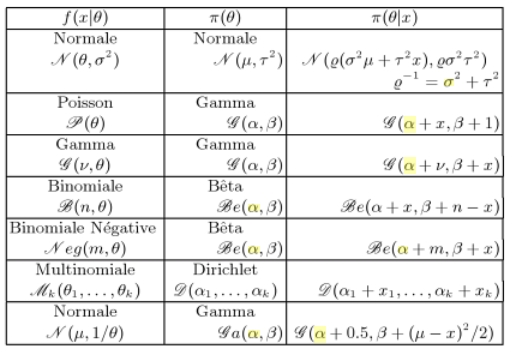
\includegraphics[scale=0.6]{figures/prior/prior.jpeg}
    \caption{Priors conjugués pour des choix de vraisemblance NEF (tiré de C.P. Robert, 2006).}
    \label{conjug}
\end{figure}

\paragraph{Intérêt de la conjugaison.} 
\begin{enumerate}
\item {\bf C'est pratique.} Le premier intérêt de la conjugaison est généralement le côté pratique : on sait directement résoudre le problème du calcul {\it a posteriori}, et généralement on connaît des algorithmes pour manipuler la famille $\Pi_{\omega}$. 
\item {\bf C'est logique.} On peut considérer que l'information $x\sim f(x|\theta)$ transformant $\pi(\theta)$ en $\pi(\theta|x)$ est limitée, donc elle ne devrait pas entra\^iner une modification de {\it toute} la \emph{structure} de $\pi(\theta)$, mais simplement de ses \emph{hyperparamètres} :
\begin{eqnarray*}
\pi(\theta) = \pi(\theta|\delta) & \Rightarrow & \pi(\theta|x) = \pi(\theta|\delta + s(x)).
\end{eqnarray*}
Cette modification devrait être de dimension finie, et un changement plus radical de $\pi(\theta)$ est peu acceptable.
\item {\bf Elle offre une interprétation claire.} En effet, si un prior conjugué existe et qu'il est exponentiel, tel
\begin{eqnarray*}
\pi(\theta|x_0,m) & \propto &  \exp\left\{\theta\cdot x_0 - m\psi(\theta)\right\} 
\end{eqnarray*} 
alors l'espérance {\it a priori prédictive} est
\begin{eqnarray*}
\E[X] & = & \E[\E[X|\theta]] \ = \ \E\left[\nabla\psi(\theta)\right] \ = \ \frac{x_0}{m}
\end{eqnarray*} 
et l'espérance {\it a posteriori prédictive}, sachant un échantillon ${\bf x_n}=(x_1,\ldots,x_n)$, est
\begin{eqnarray}
\E[X|{\bf x_n}] & = & \frac{x_0 + n\bar{x}}{m + n}. \label{linearitetototutu}
\end{eqnarray} 
Autrement dit, $m$ a le sens d'une \emph{taille d'échantillon virtuelle}, offrant une indication de la \emph{``force" informative} de l'{\it a priori} (d'un expert, etc.). Ce résultat bénéficie d'une réciprocité forte offerte par le théorème de Diaconis-Ylvisaker.
\end{enumerate}

\begin{theorem}{\bf (Diaconis-Ylvisaker).}
Si la mesure de référence est continue par rapport à la mesure de Lebesgue, alors
\begin{eqnarray*}
\E[X|{\bf x_n}] & = & \frac{x_0 + n\bar{x}}{m + n} \ \ \Rightarrow \ \ \pi(\theta|x_0,m)  \propto   \exp\left\{\theta\cdot x_0 - m\psi(\theta)\right\}.
\end{eqnarray*}
\end{theorem}

\begin{exec}{Cas multinomial.}
On considère $X|\theta$ suivant une loi multinomiale avec $X=(X_1,\ldots,X_d)$ et $\theta=(\theta_1,\ldots,\theta_{d})$ tel que
$0\leq \theta_i \leq 1$ et $\sum_{i=1}^d \theta_i=1$ :
\begin{eqnarray*}
P(X_1=k_1,\ldots,X_d=k_d|\theta) & = & \frac{n!}{k_1!\ldots k_d!} \theta^{k_1}_1\ldots \theta^{k_d}_d.  
\end{eqnarray*}
Montrer que la loi de Dirichlet est conjuguée pour cette vraisemblance.
\end{exec}

\begin{exec}{Loi inverse Wishart.}
Soient des observations $x_1,\ldots,x_n\sim{\cal{N}}_p(\mu,\Sigma)$, de loi jointe
\begin{eqnarray*}
f(x_1,\ldots,x_n|\theta=(\mu,\Sigma)) & \propto & \left(\det \Sigma\right)^{-n/2} \exp\left(-\frac{1}{2}\left[n(\bar{x}_n-\mu)^T \Sigma^{-1} (\bar{x}_n-\mu) + \mbox{tr}(\Sigma^{-1} S_n)\right]\right)
\end{eqnarray*}
avec $S_n=\sum_{i=1}^n (x_i-\bar{x}_n)(x_i-\bar{x}_n)^T$. 
On suppose prendre {\it a priori}
\begin{eqnarray*}
\mu|\Sigma & \sim & {\cal{N}}_p\left(\mu_0,\frac{1}{n_0}\Sigma\right) \\
\Sigma & \sim & {\cal{IW}}(\alpha,V) 
\end{eqnarray*} 
la loi de Wishart inverse ${\cal{IW}}$ étant définie (sur l'espace des matrices symétriques non indépendantes de rang $d$) par la densité
\begin{eqnarray*}
f(x) & = & \frac{|V|^{\alpha/2}}{2^{\alpha d/2} \Gamma_d(\alpha/2)} |x|^{-\frac{\alpha+d+1}{2}} \exp\left\{-\frac{1}{2} \text{tr}\left(V x^{-1}\right)\right\}
\end{eqnarray*}
où $\Gamma_d$ est la fonction gamma multivariée. Le prior est-il conjugué ? En dimension 1, à quelle loi se réduit-il ?
\end{exec}

\if\mycmdexothree1 \vspace{1cm} \begin{rep} % loi de Wishart
Les lois {\it a posteriori} peuvent s'écrire directement sous la forme conditionnelle
\begin{eqnarray*}
\mu|\Sigma,x_1,\ldots,x_n & \sim & {\cal{N}}_p\left( \frac{n_0 \mu_0 + n \bar{x}_n}{n_0 + n}, \frac{1}{n_0+n} \Sigma\right) \\
\Sigma| x_1,\ldots,x_n & \sim & {\cal{IW}}\left(\alpha + n, V^{-1} + S_n + \frac{nn_0}{n+n_0} (\bar{x}_n-x_0)(\bar{x}_n-x_0)^T\right).
\end{eqnarray*}
Elle est donc bien conjuguée et se réduit à un mélange gaussien - inverse gamma en dimension 1.
\end{rep}
\fi
\vspace{0.5cm}


\begin{exec}
Soit $X\sim {\cal{N}}(\theta,\theta)$ avec $\theta>0$. 
\begin{enumerate}
\item Déterminer la loi {\it a priori} de Jeffreys $\pi^J(\theta)$
\item \'Etablir si la loi de $X$ appartient à la famille exponentielle et construire les lois {\it a priori} conjuguées sur $\theta$.
\item Utiliser la propriété de linéarité des espérances des familles exponentielles pour relier les hyperparamètres des lois conjuguées à l'espérance de $\theta$.
\end{enumerate}
\end{exec}

\if\mycmdexothree1 \vspace{1cm} \begin{rep}
\begin{enumerate}
\item Avec $f(x|\theta)   \propto  \theta^{-1/2} \exp\left(-\frac{(x-\theta)^2}{2\theta} \right)$, on a donc
\begin{eqnarray*}
\log f(x|\theta) & = & - \frac{1}{2}\log\theta - (x-\theta)^2/2\theta, \\
& = & - \frac{1}{2}\log\theta - \frac{x^2}{2\theta} + x - \theta/2
\end{eqnarray*}
puis
\begin{eqnarray*}
\frac{\partial \log f(x|\theta) }{\partial \theta} & = & -\frac{1}{2\theta}  + \frac{x^2}{2\theta^2} -1/2, \\
\frac{\partial^2 \log f(x|\theta) }{\partial \theta^2} & = & -\frac{1}{2\theta^2} - \frac{x^2}{\theta^3}.
\end{eqnarray*}
Avec $\E[X]=\theta$ et $\E[X^2] = \V[X]+\E^2[X]= \theta+ \theta^2$, l'information de Fisher vaut, puisque la densité est absolument continue par rapport à $\theta\in\R^+_*$,
\begin{eqnarray*}
-\E\left[\frac{\partial^2 \log f(x|\theta) }{\partial \theta^2}(\theta)\right] & \propto & \frac{1}{\theta} + \frac{3}{2\theta^2},
\end{eqnarray*}
%qui est strictement positive si et seulement si $\theta>1/2$ 
et donc
\begin{eqnarray*}
\pi^J(\theta) & \propto &\sqrt{ \frac{1}{\theta} + \frac{3}{2\theta^2}}.
\end{eqnarray*}
\item  On peut écrire
\begin{eqnarray*}
f(x|\theta) & \propto & \theta^{-1/2} \exp\left(-\frac{(x-\theta)^2}{2\theta}\right) \ \propto \  C(\theta) h(x)  \exp\left(R(\theta)\cdot T(X)\right)
\end{eqnarray*}
avec
\begin{eqnarray*}
R(\theta) & = &  -1/\theta, \ \ \ \   T(x) \ = \ x^2/2, \\ \\
h(x) & = & \exp(x), \ \ \ \  \ 
C(\theta)  \ = \  \exp(-\log(\theta)/2 - \theta/2)
\end{eqnarray*}
ce qui correspond à l'écriture canonique des lois exponentielles :
\begin{eqnarray*}
f(x|\theta) & = & C(\theta) h(x) \exp\left(R(\theta)\cdot T(X)\right).
\end{eqnarray*}
Nous souhaiterions arriver à l'écriture suivante : pour une reparamétrisation $z$ de $x$ et une reparamétrisation  $\eta$ de $\theta$, 
\begin{eqnarray}
Z|\eta & \sim & f(z|\theta) \ = \ h(z) \exp\left(\eta\cdot z - \psi(\eta) \right) \label{conjugaison}
\end{eqnarray}
afin de proposer la  famille de priors  conjugués :
\begin{eqnarray*}
\pi(\eta) & \propto & \exp\left(\eta \cdot z_0 - \psi(\eta) \right). 
\end{eqnarray*}
Essayons avec la reparamétrisation $\eta  =  1/\theta$ et $z  =  x^2/2$ 
 (on se restreint donc à $\R^+$) et on peut alors écrire
\begin{eqnarray*}
\psi(\eta) & = & \log \int_0^{\infty}  h(z) \exp\left(\eta\cdot z\right) \ dz
\end{eqnarray*}
Il faut ici écrire $h(z)$ proprement, puis définir $\pi(\eta)$ puis enfin $\pi(\theta)$. 
\end{enumerate}
\end{rep}
\fi
\vspace{0.5cm}

\paragraph{\bf Modèles de mélange.} La conjugaison peut s'étendre à des modèles de mélange. En effet, soit ${\cal{F}}=\{\pi(\theta|a,b)=K(a,b)\exp(\theta\cdot a - b\psi(\theta))\}$  la famille conjuguée naturelle de la famille exponentielle
\begin{eqnarray*}
f(x|\theta) & = & C(\theta)h(x)\exp(\theta\cdot x).
\end{eqnarray*}
Alors l'ensemble des mélanges de $N$ lois conjuguées
\begin{eqnarray*}
{\cal{F}}_N & = & \left\{\sum\limits_{i=1}^N \omega_i\pi(\theta|a_i,b_i); \sum\limits_{i=1}^N \omega_i=1, \ \omega_i>0\right\}
\end{eqnarray*}
est aussi une famille conjuguée.  
{\it A posteriori}, on a
\begin{eqnarray*}
\pi(\theta|x) & = & \sum\limits_{i=1}^N \omega'_i(x)\pi(\theta|a_i+1,b_i+x)
\end{eqnarray*}
avec
\begin{eqnarray*}
\omega'_i(x) & = & \frac{\omega_i K(a_i,b_i)/K(a_i+1,b_i+x)}{\sum_{j=1}^N \omega_j K(a_j,b_j)/K(a_j+1,b_j+x)}. 
\end{eqnarray*}


Les \emph{mélanges d'{\it a priori} conjugués} peuvent alors \^etre utilisés comme \emph{base pour approcher une loi {\it a priori} quelconque}, au sens où la distance de Prohorov entre une loi  et sa représentation par un mélange dans ${\cal{F}}_N$ peut \^etre rendue arbitrairement petite. Cela fournit un argument fort en faveur de l'utilisation des lois conjuguées. 

\begin{definition}{\bf Distance de Prohorov.}
La distance de \emph{Prohorov} entre deux mesures $\pi$ et $\tilde{\pi}$ est définie par
\begin{eqnarray*}
D^p(\pi,\tilde{\pi}) & = & \inf\limits_{A}\left\{ \epsilon ; \ \pi(A)\leq \tilde{\pi}(A^{\epsilon}) + \epsilon\right\}
\end{eqnarray*}
où l'infimum est pris sur les ensembles boréliens de $\Theta$ et où $A^{\epsilon}$ indique l'ensemble des points distants de $A$ d'au plus $\epsilon$.
\end{definition}

\begin{theorem}
Pour toute loi {\it a priori} $\pi$ sur $\Theta$, 
$\forall \epsilon>0$, on peut trouver $N$ et $\tilde{\pi}\in{\cal{F}}_N$ tel que
\begin{eqnarray*}
D^p(\pi,\tilde{\pi}) & < & \epsilon. 
\end{eqnarray*}
\end{theorem}

\paragraph{Au-delà de la famille exponentielle.} Le mécanisme de conjugaison n'est pas réservé aux lois de la famille exponentielle. Par exemple, la loi de Pareto avec $\alpha>0$ connu, et $\theta>0$, de densité
\begin{eqnarray*}
f(x|\theta) & = & \alpha\frac{\theta^\alpha}{x^{\alpha+1}}\1_{]\theta,\infty[}(x),
\end{eqnarray*}
admet un {\it a priori} conjugué, qui est Pareto sur $1/\theta$. 

\begin{exec}
Considérons les deux lois uniformes de densité
\begin{eqnarray*}
f(x|\theta) & = & \frac{\1_{[-\theta,\theta]}(x)}{2\theta} \\
f(x|\theta) & = & \frac{\1_{[Con0,\theta]}(x)}{\theta}.
\end{eqnarray*}
Admettent-elles des priors conjugués ?
\end{exec}

%%%%%%%%%%%%%%%%%%%%%%%%%%%%%%
%\subsection{Au-delà des cas conjugués : l'approche subjectiviste}


%%%%%%%%%%%%%%%%%%%%%%%%%%%%%%
\subsection{Priors hiérarchiques}

Pour des raisons liées à la modélisation des observations ou à la décomposition de l'information {\it a priori}, le modèle bayésien $(f(x|\theta), \pi(\theta))$ peut \^etre défini comme \emph{hiérarchique} : $\pi(\theta)$ est décomposé en plusieurs {\it lois conditionnelles}
\begin{eqnarray*}
{\pi(\theta|\theta_1,\ldots,\theta_{k})} & = & {\pi_1(\theta|\theta_1)\cdots\pi_2(\theta_1|\theta_2)\ldots \pi_k(\theta_{k-1}|\theta_k)\cdot\pi_{k+1}(\theta_k)} \\
\text{et} \ \ \ \ \pi(\theta) & = & \int_{\Theta_1\times\ldots\times\Theta_k} \pi(\theta|\theta_1,\ldots,\theta_{k}) \ d\theta_1\ldots d\theta_k. \\
\end{eqnarray*}

\begin{exo}{\it Modèle linéaire à effets aléatoires:}
\begin{eqnarray*}
y|\theta & \sim & {\cal{N}}_p(\theta,\Sigma_1), \\
\theta|\beta & \sim & {\cal{N}}_p(X\beta,\Sigma_2)
\end{eqnarray*}
souvent utilisé en génétique animale pour différencier l'influence d'éléments fixes (ex: lignée, race, année) de celle de facteurs aléatoires (ex : nb de femelles dans une lignée).
\end{exo}

\paragraph{\bf Conditionnement.} Le conditionnement peut apparaître par 
\begin{itemize}
\item des \emph{dépendances statistiques naturelles} ; 
\item l'appel à des \emph{variables latentes} décrivant un \emph{mécanisme caché} ; 
\item des grandeurs stochastiques jouant un r\^ole de \emph{for\c cage}. 
\end{itemize}
En général, on ne va guère plus loin que deux ou trois niveaux de hiérarchie. En incluant l'information {\it a priori} aux niveaux les plus élevés, l'approche bayésienne hiérarchique permet en général de gagner en \emph{robustesse}. \\

\paragraph{\bf Exemples de conditionnements naturels.} Ces conditionnements peuvent apparaître à partir de résultats statistiques théoriques. \\

\begin{exo}
La \emph{courbe de von Bertalanffy} 
\begin{eqnarray*}
L(t|\theta) & = & L_{\infty}(1 - exp(-g(t,\delta)) 
\end{eqnarray*}
est fréquemment utilisée pour produire une {\bf clé \^age-longueur}, en modélisant l'accroissement en longueur d'un organisme vivant (ex: arbre, poisson...). On note $\theta=(L_{\infty},\delta)$ le vecteur des paramètres inconnus. Supposons disposer de données de capture-recapture, càd des couples d'observation $\left\{l^*(t_i),l^*(t_{i+\Delta_i})\right\}$ tel que
\begin{eqnarray*}
l^*(t_i) & = & L(t_i|\theta)\exp(\epsilon_1), \\
l^*(t_{i+\Delta_i}) & = & L(t_i+\Delta_i|\theta)\exp(\epsilon_2)
\end{eqnarray*}
où $(\epsilon_1,\epsilon_2)$ sont des \emph{bruits de mesure} (générant donc une vraisemblance). Les estimations par maximum de vraisemblance de  $L_{\infty}$ étant très sensibles à la taille des données, on cherche donc à produire un prior sur  $L_{\infty}$. On peut tirer parti du théorème de Pickands en comprenant que $L_{\infty}$ peut être assimilé à une longueur maximale qu'un être vivant peut atteindre, en moyenne sur toutes les observations possibles. Posons alors $L^*_{\infty} = L_{\infty}\exp(\epsilon)$ la longueur maximale {\it observée}. Soit $\bar{L}$ la longueur moyenne.  On obtient alors une justification pour :
\begin{enumerate}
\item établir une forme {\it a priori} pour $\pi(L_{\infty})$ (la forme de $\epsilon$ étant fixée) ; 
\item conditionner ce prior par rapport à $\bar{L}$ $\Leftrightarrow$ utiliser une \emph{approche bayésienne hiérarchique}. 
\end{enumerate}  
\end{exo}

\begin{theorem}{\bf Pickands (1975).} 
Quand $\bar{L}$ grandit, la distribution de $L^*_{\infty}|\bar{L}=l$ est une loi de Pareto généralisée :
\begin{eqnarray*}
P\left(L^*_{\infty}<x|L^*_{\infty}>\bar{L},\sigma,\mu\right) & = & 1 - \left( 1 + \mu\left(\frac{x-\bar{L}}{\sigma}\right)\right)^{-1/\mu} 
\end{eqnarray*}
\end{theorem}

\begin{exo}
Soit $X_t$ un nombre d'individus dans une population. Soit $\theta=\theta_{t,t+1}$ la probabilité de survie entre $t$ et $t+1$. La vraisemblance de ces données markoviennes peut être définie par le noyau de transition 
\begin{eqnarray*}
X_{t+1}|X_t,\theta_{t,t-1} & \sim & {\cal{B}}(X_t,\theta_{t,t+1}) \ \ \ \text{\it (loi binomiale)}
\end{eqnarray*}
 On peut alors écrire
\begin{eqnarray*}
\theta_{t,t+1} & = & \prod_{i=0}^{M+1} \theta_{t+i/M,t+(i+1)/M}
\end{eqnarray*}
donc, de par le Théorème de la Limite Centrale, quand $1\ll M$,
\begin{eqnarray*}
\log(\theta_{t,t+1}) & \sim & {\cal{N}}(\mu_t,\sigma^2_t)
\end{eqnarray*}
avec $\mu_t<-\sigma^2_t/2$ tel que $\E[\theta_{t,t+1}] \in[0,1]$ qui est une contrainte de  forme sur le niveau hiérarchique $\pi(\mu_t,\sigma_t)$.
\end{exo}

\paragraph{Graphes acycliques orientés.} On peut représenter les causalités et dépendences probabilistes sous forme de graphes acycliques orientés (DAG = {\it direct acyclic graphs}, cf. figures \ref{DAG1}-\ref{DAG2}). Ce type de représentation peut s'avérer utile pour l'encodage sous certains logiciels (famille BUGS) et pour s'assurer de la cohérence interne d'un modèle bayésien hiérarchique. Dans ce type de représentation, les informations connues (typiquement : les données) sont représentées sous la forme de rectangles) tandis que les variables aléatoires sont placées dans des ellipses (ex : figure \ref{DAG3}).

\begin{figure}[h!]
\centering
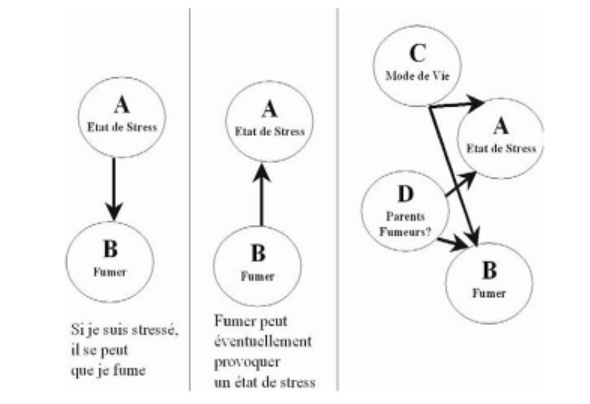
\includegraphics[scale=0.4]{figures/prior/parent1.jpeg}
\caption{DAG tiré de Parent et Bernier (2007). }
\label{DAG1}
\end{figure}

\begin{figure}[h!]
\centering
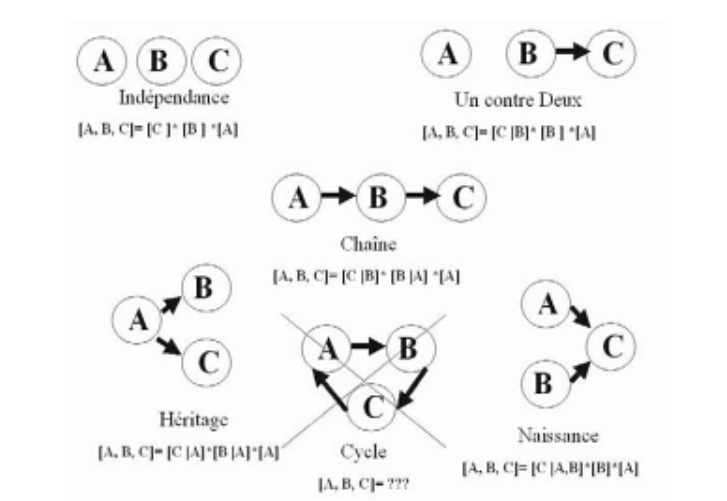
\includegraphics[scale=0.4]{figures/prior/parent2.jpeg}
\caption{Relations de dépendance conditionnelles possibles entre trois variables aléatoires. DAG tiré de Parent et Bernier (2007). }
\label{DAG2}
\end{figure}


\begin{figure}[h!]
\centering
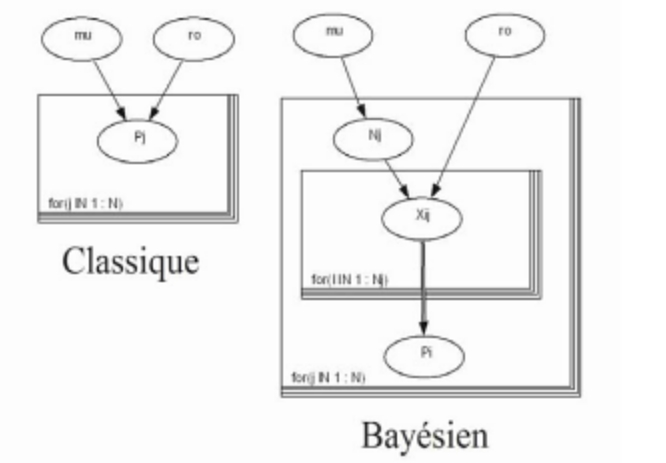
\includegraphics[scale=0.4]{figures/prior/parent3.jpeg}
\caption{DAG incluant des variables latentes. DAG tiré de Parent et Bernier (2007). }
\label{DAG3}
\end{figure}

\subsubsection{Un exemple utile : les \emph{Latent Gaussian Models} (LGM)}

On note $Y_i$ la variable réponse, reliée à $\mu_i$ par 
\begin{eqnarray*}
Y_i & = & {\cal{N}}(\mu_i,\sigma^2)
\end{eqnarray*}
où $\mu_i$ est tel que 
$$
g(\mu_i) = \eta_i = \alpha + \sum\limits_j f^j(u_{i,j}) + \sum\limits_k \beta_k Z_{k,i} + \varepsilon_i.
$$


\clearpage
%%%%%%%%%%%%%%%%%%%%%%%%%%%%%%
\subsection{Convergence des priors informatifs vers des priors régularisant}

On peut interpréter, et édifier comme une règle de bon sens permettant de juger le bien-fondé d'un prior informatif, le fait qu'un {\it a priori} régularisant, typiquement impropre, soit décrit comme la limite d'une suite de priors informatifs \emph{en un certain sens} (de moins en moins informatifs). Ce "sens" a fait l'objet de nombreuses spéculations au cours du temps, et a été définitivement formalisé dans les travaux de Bioche (2015). \\

\begin{exo}
Soit $X\sim {\cal{E}}(\lambda)$ et $\pi(\lambda)\equiv {\cal{G}}(a,b)$. On sait alors que la loi {\it a posteriori} de $\lambda$ sachant un échantillon iid  $x_1,\ldots,x_n$ est $\lambda\sim{\cal{G}}(a+n,b+\sum_{i=1}^n x_i)$. Les hyperparamètres $(a,b)$ ont le sens respectif d'une taille et d'une somme d'échantillon virtuel. "Moralement", faire tendre $(a,b)$ vers 0 revient à annuler l'information apportée par cet échantillon virtuel. On voit alors que $\forall \lambda>0$, $\pi(\lambda)$ "tend" vers $1/\lambda$, qui est bien le prior de Jeffreys.  \\
\end{exo}

Ainsi, Wallace (1959) a proposé une première démarche s'appuyant sur la convergence en tout point : 

\begin{proposition}
Si $\pi$ est une densité {\it a priori} impropre, alors  il existe une suite de densités {\it a priori} propres $\{\pi_n\}_n$ 
engendrant une suite d'{\it a posteriori} $\{{\pi_n}(.|x)\}_n$ telle que pour tout  $\theta\in\Theta$ et pour tout $x$,
tout $x$,
$$
\lim\limits_{n \to \infty} {\pi_n} (\theta |x)  =  \pi(\theta |x).
$$
Ce résultat reste vrai si $\{{\pi_n}\}_n$  est une suite de densités telle qu'il existe une constante $K$ et une suite $\{{a_n}\}_n$ telle que, pour tout $\theta$,
$$
\lim\limits_{n \to \infty} a_n {\pi_n}(\theta)  =  \pi(\theta) \ \ \ \  \text{et} \ \ \ \  a_n {\pi_n}(\theta) \leq K  \pi(\theta).
$$
\end{proposition}

Comme l'a fait remarquer Stone en 1965, ce type d'approche est \emph{rétrospective} : le jeu de données est fixé avant tout. Or on souhaite pouvoir caractériser le comportement de $\pi(\theta)$ \emph{avant} l'occurence de données. D'autres notions de convergence de mesures ont été pour cela étudiées.
\begin{enumerate}
\item La \emph{convergence en probabilité} proposée par Stone (1965) vers des mesures impropres {\it relativement invariantes}   continues et  
telles que $\pi(\theta_1,\theta_2) = \pi(\theta_1)\pi(\theta_2)$ . Cette approche nécessite d'introduire des suites de mesures {\it a priori} obtenues par troncature (suite croissante de compacts sur $\Theta$).
 \item La \emph{convergence en variation totale} considérée par Head et Sudderth (1989), définie par
\begin{eqnarray*}
\| \pi_n(\theta) - \pi(\theta) \| & = & \sup\limits_{{\cal{F}}} | \pi_n(\theta) - \pi(\theta) |
\end{eqnarray*}  
où ${\cal{F}}$ est une $\sigma-$algèbre de sous-ensembles de $\Theta$.
\item La \emph{convergence en entropie relative} étudiée par Berger et ses co-auteurs en 2009. \\
\end{enumerate}
Mais ces approches supposent de nombreuses hypothèses et n'offrent pas une vision complète de la convergence. En particulier, elles nécessitent souvent de travailler sur des suites de sous-ensembles de $\Theta$ compacts, des priors tronqués, et les lois {\it a posteriori} limites ne sont pas forcément cohérents avec les mesures régularisantes obtenues par des règles formelles. \\

Ainsi, Bioche (2015) est la première à proposer une vision {\it prospective} ou intrinsèque (préalable à l'occurence de données) complète, par le biais de la \emph{convergence vague} des mesures de Radon strictement positives (soit des mesures strictement positives finies sur les compacts). Ce mode de convergence est équivalent à la notion de \emph{convergence étroite} pour les mesures bornées (et donc les mesures de probabilité).

\begin{definition}{\bf Convergence vague de mesures de Radon.}
Soit $\{\mu_n\}_n$  et $\mu$ des mesures (de Radon). La suite $\{\mu_n\}_n$ converge
vaguement vers $\mu$ si,  pour toute fonction $h$ continue à support compact, 
\begin{eqnarray*}
\lim\limits_{n\to\infty} \int h d\mu_n & = & \int h d\mu.
\end{eqnarray*}
\end{definition}

\begin{definition}{\bf Convergence étroite de mesures bornées.}
Soit $\{\mu_n\}_n$  et $\mu$ des mesures bornées. La suite $\{\mu_n\}_n$ converge
étroitement vers $\mu$ si,  pour toute fonction $h$ continue bornée, 
\begin{eqnarray*}
\lim\limits_{n\to\infty} \int h d\mu_n & = & \int h d\mu.
\end{eqnarray*}
\end{definition}

\`A partir de ces ingrédients, on peut définir la \emp{$q-$convergence vague} de mesures positives. 

\begin{definition}{\bf $q-$convergence vague de mesures positives.}
Une suite de mesures positives $\{\mu_n\}_n$ converge $q-$vaguement vers une mesure positive $\mu$ s'il existe une suite de réels positifs $\{a_n\}_n$ telle que $\{a_n \mu_n\}_n$ converge vaguement vers $\mu$. 
\end{definition}

On obtient alors le résultat suivant. \\

\begin{proposition}
Si $(\pi_n)_n$ est une suite de priors qui converge $q-$vaguement vers $\pi$, et si $\theta\to f(x|\theta)$ est une fonction continue sur $\Theta$ et non nulle, alors $\pi_n(.|x)$ converge $q-$vaguement vers $\pi(.|x)$.
\end{proposition}

\noindent {Dans les cas discrets}, si $\mu$ et $\mu_n$ sont définies sur $\Theta=\{\theta_i\}_{i\in I}$, la convergence $q-$vague est équivalente à : $\forall i\in I$, 
$$
\lim\limits_{n\to\infty} a_n \mu_n(\theta_i) = \mu(\theta_i).
$$
{ Dans les cas continus}, on peut obtenir le résultat suivant. 

\begin{proposition}\label{condition.continue}
Soient $\mu$ et $\mu_n$ des mesures {\it a priori} sur $\Theta$. Supposons que :
\begin{enumerate}
\item il existe un suite de réels positifs $\{a_n\}_n$ tel que la suite $\{a_n \mu_n\}_n$ converge ponctuellement vers $\mu$ ; 
\item pour tout ensemble compact $K$, il existe un scalaire $M$ et $N\in\N$ tels que, pour tout $n>N$, 
$$
\sup_{\theta\in K} a_n \mu_n(\theta) < M.
$$
\end{enumerate}
Alors $\{\mu_n\}_n$ converge $q-$vaguement vers $\mu$.
\end{proposition}

\begin{exec}
Soit $\Theta=\N$ et $\Pi_n= {\cal{U}}\left(\left\{0,1,\ldots,n\right\}\right)$ la distribution uniforme discrète sur le compact discret $\{0,\ldots,n\}$.  Prouver que $\{\Pi_n\}_n$ converge $q-$vaguement vers la mesure de comptage.
\end{exec}

\if\mycmdexothree1 \vspace{1cm} \begin{rep} % Exercice de convergence q-vague de la distribution uniforme discrète vers la mesure de comptage
On a 
\begin{eqnarray*}
\pi_n(\theta) & = & \frac{1}{n+1}\1_{\{0,1,\ldots,n\}}(\theta).
\end{eqnarray*}
Choisissons $a_n=n+1$. Alors pour tout $\theta\in\N$, $\lim_{n\to\infty} a_n \pi_n(\theta) = \lim_{n\to\infty} \1_{\{0,1,\ldots,n\}}(\theta) = 1$. 
\end{rep}
\fi
\vspace{0.5cm}


%\begin{exec}
%Soit $\Theta=\R$ et $\Pi_n= {\cal{U}}\left([-n,n]\right)$. Prouver que $\{\Pi_n\}_n$ converge $q-$vaguement vers la mesure de Lebesgue.
%\end{exec}

%\if\mycmdexothree1 \vspace{1cm} \begin{rep} % Exercice de convergence q-vague de la distribution uniforme continue vers la mesure de Lebesgue

\end{rep}
%\fi
%\vspace{0.5cm}

\begin{exec}
Soit $\Theta=\R$ et $\Pi_n= {\cal{N}}(0,n)$. Prouver que $\{\Pi_n\}_n$ converge $q-$vaguement vers la mesure de Lebesgue.
\end{exec}

\if\mycmdexothree1 \vspace{1cm} \begin{rep} % Exercice de convergence q-vague de la distribution gaussienne centrée  vers la mesure de Lebesgue
On a
\begin{eqnarray*}
\pi_n(\theta) & = & \frac{1}{\sqrt{2\pi n}}\exp\left(-\theta^2/2n\right).
\end{eqnarray*}
et $\pi(\theta)=1$. 
Choisissons $a_n=\sqrt{2\pi n}$ pour $n>0$. Alors pour tout $\theta\in\N$, $\lim_{n\to\infty} a_n \pi_n(\theta) = 1$. De plus, $\forall (n,\theta)$, $a_n\pi_n(\theta)<2$. On utilise ensuite la proposition \ref{condition.continue}.  
\end{rep}
\fi
\vspace{0.5cm}





